In this section we include multiple examples on defining and simulating models.

\hyperlink{example_events}{Example Events} \+: Forward Sensitivities for model with events and discontinuities.

\hyperlink{example_dirac}{Example Dirac} \+: Forward Sensitivities for m\+R\+N\+A transfection model with bolus injection.

\hyperlink{example_steadystate}{Example Steady State} \+: Steady State Sensitivities.

\hyperlink{example_jakstat_adjoint}{Example J\+A\+K/\+S\+T\+A\+T Adjoint} \+: Adjoint Sensitivities for J\+A\+K/\+S\+T\+A\+T model with parametric standard deviation.

\hyperlink{example_dirac_adjoint}{Example Dirac Adjoint} \+: Adjoint Sensitivities for m\+R\+N\+A transfection model with bolus injection.

\hyperlink{example_dirac_secondorder}{Example Dirac Second Order Forward} \+: Second order forward sensitivities for m\+R\+N\+A transfection model with bolus injection.

\hyperlink{example_dirac_secondorder_vectmult}{Example Dirac Directional Second Order Forward} \+: Directional second order forward sensitivities for m\+R\+N\+A transfection model with bolus injection.

\hyperlink{example_adjoint}{Example Adjoint} \+: Adjoint Sensitivities for simple model with analytic solution. \hypertarget{example_events}{}\subsection{Example Events}\label{example_events}
\hypertarget{example_events_def_events}{}\subsubsection{Model Definition}\label{example_events_def_events}
 
% This LaTeX was auto-generated from MATLAB code.
% To make changes, update the MATLAB code and republish this document.











    
    \begin{DoxyCode}
function [model] = model_events_syms()
\end{DoxyCode}
\begin{DoxyCode}
% set the parametrisation of the problem options are 'log', 'log10' and
% 'lin' (default).
model.param = 'log10';
\end{DoxyCode}
\begin{par}
STATES
\end{par} \vspace{1em}
\begin{DoxyCode}
% create state syms
syms x1 x2 x3

% create state vector
model.sym.x = [
x1 x2 x3
];
\end{DoxyCode}
\begin{par}
PARAMETERS ( for these sensitivities will be computed )
\end{par} \vspace{1em}
\begin{DoxyCode}
% create parameter syms
syms p1 p2 p3 p4

% create parameter vector
model.sym.p = [p1,p2,p3,p4];

% set the parametrisation of the problem options are 'log', 'log10' and
% 'lin' (default).
model.param = 'log10';
\end{DoxyCode}
\begin{par}
CONSTANTS ( for these no sensitivities will be computed ) this part is optional and can be ommited
\end{par} \vspace{1em}
\begin{DoxyCode}
% create parameter syms
syms k1 k2 k3 k4

% create parameter vector
model.sym.k = [k1 k2 k3 k4];
\end{DoxyCode}
\begin{par}
SYSTEM EQUATIONS
\end{par} \vspace{1em}
\begin{DoxyCode}
% create symbolic variable for time
syms t

model.sym.xdot = sym(zeros(size(model.sym.x)));

% piecewise defined function
model.sym.xdot(1) = -p1*heaviside(t-p4)*x1;
% inhomogeneous
model.sym.xdot(2) = +p2*x1*exp(-0.1*t)-p3*x2 ;
model.sym.xdot(3) = -1.5*x3;
\end{DoxyCode}
\begin{par}
INITIAL CONDITIONS
\end{par} \vspace{1em}
\begin{DoxyCode}
model.sym.x0 = sym(zeros(size(model.sym.x)));

model.sym.x0(1) = k1;
model.sym.x0(2) = k2;
model.sym.x0(3) = k3;
\end{DoxyCode}
\begin{par}
OBSERVALES
\end{par} \vspace{1em}
\begin{DoxyCode}
model.sym.y = sym(zeros(1,1));

model.sym.y(1) = p4 * (x1+x2+x3);
\end{DoxyCode}
\begin{par}
EVENTS this part is optional and can be ommited
\end{par} \vspace{1em}
\begin{DoxyCode}
syms t

% events fire when there is a zero crossing of the root function
model.event(1) = amievent(x3-x2,0,t);
model.event(2) = amievent(x3-x1,0,t);
\end{DoxyCode}
\begin{DoxyCode}
end
\end{DoxyCode}

         \begin{DoxyCode}ans = 
    param: 'log10'
      sym: [1x1 struct]
    event: [1x2 amievent]
\end{DoxyCode} 
    



    \hypertarget{example_events_simu_events}{}\subsubsection{Simulation}\label{example_events_simu_events}
 
% This LaTeX was auto-generated from MATLAB code.
% To make changes, update the MATLAB code and republish this document.











    
    \begin{DoxyCode}
function example_events()
\end{DoxyCode}
\begin{par}
COMPILATION
\end{par} \vspace{1em}
\begin{DoxyCode}
[exdir,~,~]=fileparts(which('example_events.m'));
% compile the model
amiwrap('model_events','model_events_syms',exdir)
\end{DoxyCode}

         \begin{DoxyCode}Generating model struct ...
Parsing model struct ...

Generating C code ...
headers | wrapfunctions | 
Compiling mex file ...
amici | Building with 'Xcode with Clang'.
MEX completed successfully.
Building with 'Xcode with Clang'.
MEX completed successfully.
\end{DoxyCode} 
    \begin{par}
SIMULATION
\end{par} \vspace{1em}
\begin{DoxyCode}
% time vector
t = linspace(0,10,20);
p = [0.5;2;0.5;0.5];
k = [4,8,10,4];

options = amioption('sensi',0,...
    'maxsteps',1e4,...
    'nmaxevent', 2);
D = amidata(length(t),1,2,2,4);
% load mex into memory
[~] = which('simulate_model_events'); % fix for inaccessability problems
sol = simulate_model_events(t,log10(p),k,D,options);

tic
sol = simulate_model_events(t,log10(p),k,D,options);
disp(['Time elapsed with cvodes: ' num2str(toc) ])
\end{DoxyCode}

         \begin{DoxyCode}Time elapsed with cvodes: 0.0037064
\end{DoxyCode} 
    \begin{par}
ODE15S
\end{par} \vspace{1em}
\begin{DoxyCode}
ode_system = @(t,x,p,k) [-p(1)*heaviside(t-p(4))*x(1);
    +p(2)*x(1)*exp(-0.1*t)-p(3)*x(2);
    -1.5*x(3)];
% event_fn = @(t,x) [x(3) - x(2);
%     x(3) - x(1)];
% 'Events',event_fn
options_ode15s = odeset('RelTol',options.rtol,'AbsTol',options.atol,'MaxStep',options.maxsteps);

tic
[~, X_ode15s] = ode15s(@(t,x) ode_system(t,x,p,k),t,k(1:3),options_ode15s);
disp(['Time elapsed with ode15s: ' num2str(toc) ])
\end{DoxyCode}

         \begin{DoxyCode}Time elapsed with ode15s: 0.074866
\end{DoxyCode} 
    \begin{par}
PLOTTING
\end{par} \vspace{1em}
\begin{DoxyCode}
figure
c_x = get(gca,'ColorOrder');
subplot(2,2,1)
for ix = 1:size(sol.x,2)
    plot(t,sol.x(:,ix),'.-','Color',c_x(ix,:))
    hold on
    plot(t,X_ode15s(:,ix),'d','Color',c_x(ix,:))
end
stem(sol.z(:,1),sol.z(:,1)*0+10,'r')
stem(sol.z(:,2),sol.z(:,2)*0+10,'k')
legend('x1','x1_{ode15s}','x2','x2_{ode15s}','x3','x3_{ode15s}','x3==x2','x3==x1','Location','NorthEastOutside')
legend boxoff
xlabel('time t')
ylabel('x')
box on
subplot(2,2,2)
plot(t,abs(sol.x-X_ode15s),'--')
set(gca,'YScale','log')
legend('error x1','error x2','error x3','Location','NorthEastOutside')
legend boxoff
ylabel('x')

subplot(2,2,3)
plot(t,sol.y,'.-','Color',c_x(1,:))
hold on
plot(t,p(4)*sum(X_ode15s,2),'d','Color',c_x(1,:))
legend('y1','y1_{ode15s}','Location','NorthEastOutside')
legend boxoff
xlabel('time t')
ylabel('y')
box on

subplot(2,2,4)
plot(t,abs(sol.y-p(4)*sum(X_ode15s,2)),'--')
set(gca,'YScale','log')
legend('error y1','Location','NorthEastOutside')
legend boxoff
xlabel('time t')
ylabel('y')
box on

set(gcf,'Position',[100 300 1200 500])
\end{DoxyCode}

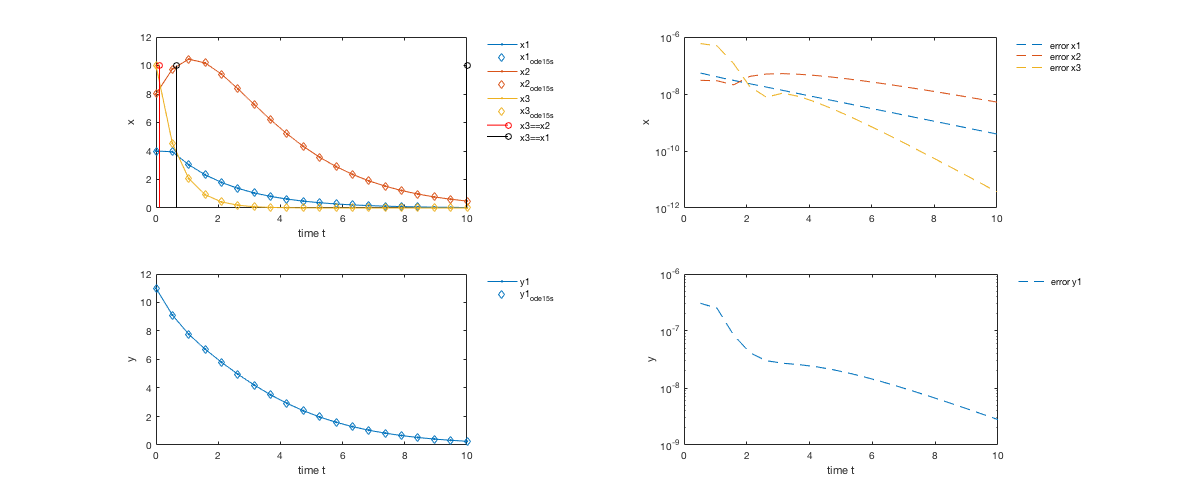
\includegraphics[width=\textwidth]{../../examples/example_events/html/example_events_01.png}
\begin{par}
FORWARD SENSITIVITY ANALYSIS
\end{par} \vspace{1em}
\begin{DoxyCode}
options.sensi = 1;

sol = simulate_model_events(t,log10(p),k,D,options);
\end{DoxyCode}
\begin{par}
FINITE DIFFERENCES
\end{par} \vspace{1em}
\begin{DoxyCode}
eps = 1e-4;
xi = log10(p);
for ip = 1:4;
    xip = xi;
    xip(ip) = xip(ip) + eps;
    solp = simulate_model_events(t,xip,k,D,options);
    sx_fd(:,:,ip) = (solp.x - sol.x)/eps;
    sy_fd(:,:,ip) = (solp.y - sol.y)/eps;
    sz_fd(:,:,ip) = (solp.z - sol.z)/eps;
end
\end{DoxyCode}
\begin{par}
PLOTTING
\end{par} \vspace{1em}
\begin{DoxyCode}
figure
for ip = 1:4
    subplot(4,2,ip*2-1)
    hold on
    for ix = 1:size(sol.x,2)
        plot(t,sol.sx(:,ix,ip),'.-','Color',c_x(ix,:))
        plot(t,sx_fd(:,ix,ip),'d','Color',c_x(ix,:))
    end
    legend('sx1','sx1_{fd}','sx2','sx2_{fd}','sx3','sx3_{fd}','Location','NorthEastOutside')
    legend boxoff
    title(['state sensitivity for p' num2str(ip)])
    xlabel('time t')
    ylabel('sx')
    box on

    subplot(4,2,ip*2)
    plot(t,abs(sol.sx(:,:,ip)-sx_fd(:,:,ip)),'--')
    legend('error sx1','error sx2','error sx3','Location','NorthEastOutside')
    legend boxoff
    title(['state sensitivity for p' num2str(ip)])
    xlabel('time t')
    ylabel('error')
    set(gca,'YScale','log')
    box on
end
set(gcf,'Position',[100 300 1200 500])

figure
for ip = 1:4
    subplot(4,2,ip*2-1)
    hold on
    for iy = 1:size(sol.y,2)
        plot(t,sol.sy(:,iy,ip),'.-','Color',c_x(iy,:))
        plot(t,sy_fd(:,iy,ip),'d','Color',c_x(iy,:))
    end
    legend('sy1','sy1_fd','Location','NorthEastOutside')
    legend boxoff
    title(['observable sensitivity for p' num2str(ip)])
    xlabel('time t')
    ylabel('sy')
    box on

    subplot(4,2,ip*2)
    plot(t,abs(sol.sy(:,:,ip)-sy_fd(:,:,ip)),'--')
    legend('error sy1','Location','NorthEastOutside')
    legend boxoff
    title(['error observable sensitivity for p' num2str(ip)])
    xlabel('time t')
    ylabel('error')
    set(gca,'YScale','log')
    box on
end
set(gcf,'Position',[100 300 1200 500])

figure
for ip = 1:4
subplot(4,2,2*ip-1)
bar(1:options.nmaxevent,sol.sz(1:options.nmaxevent,:,ip),0.8)
hold on
bar(1:options.nmaxevent,sz_fd(1:options.nmaxevent,:,ip),0.4)
legend('x3==x2','x3==x1','x3==x2 fd','x3==x1 fd','Location','NorthEastOutside')
legend boxoff
title(['event sensitivity for p' num2str(ip)])
xlabel('event #')
ylabel('sz')
box on

subplot(4,2,2*ip)
bar(1:options.nmaxevent,sol.sz(1:options.nmaxevent,:,ip)-sz_fd(1:options.nmaxevent,:,ip),0.8)
legend('error x3==x2','error x3==x1','Location','NorthEastOutside')
legend boxoff
title(['error event sensitivity for p' num2str(ip)])
xlabel('event #')
ylabel('sz')
box on
end
set(gcf,'Position',[100 300 1200 500])

drawnow
\end{DoxyCode}

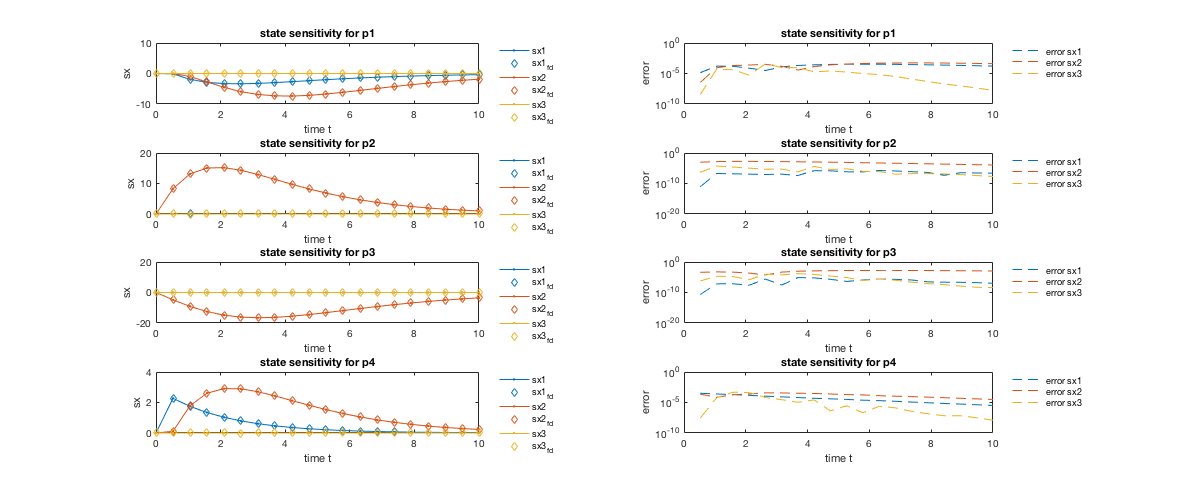
\includegraphics[width=\textwidth]{../../examples/example_events/html/example_events_02.png}

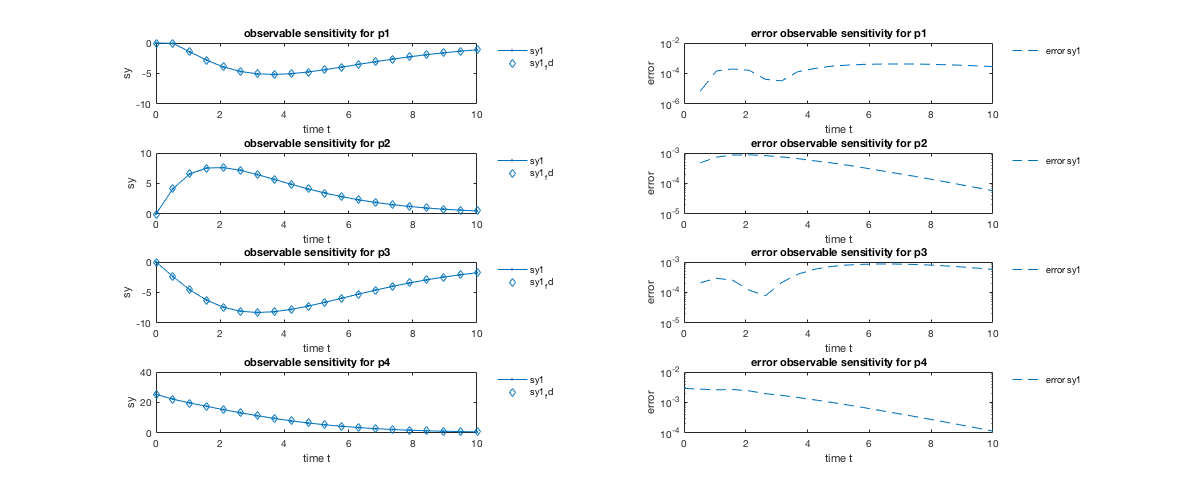
\includegraphics[width=\textwidth]{../../examples/example_events/html/example_events_03.png}

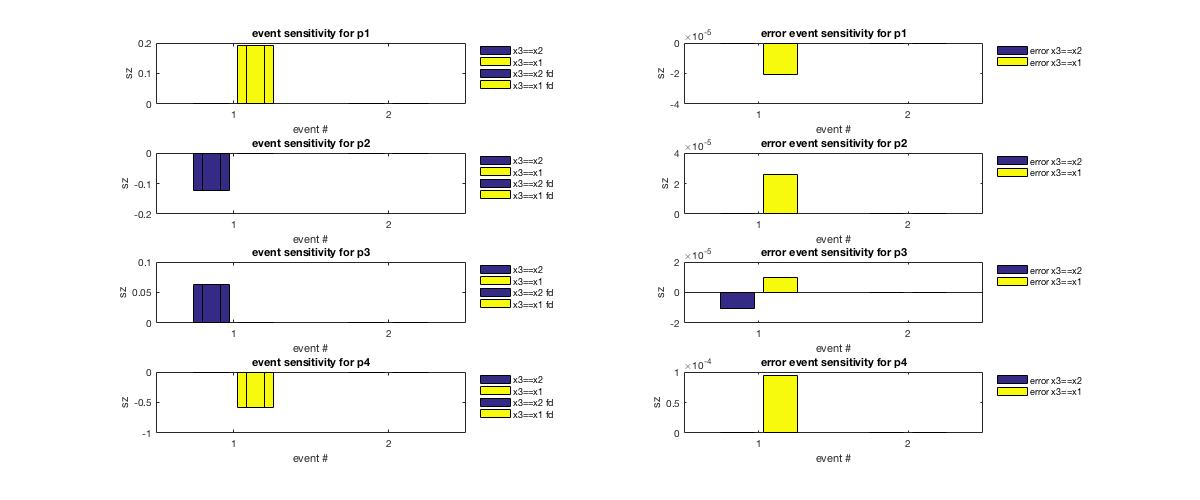
\includegraphics[width=\textwidth]{../../examples/example_events/html/example_events_04.png}
\begin{DoxyCode}
end
\end{DoxyCode}




     \hypertarget{example_dirac}{}\subsection{Example Dirac}\label{example_dirac}
\hypertarget{example_dirac_def_dirac}{}\subsubsection{Model Definition}\label{example_dirac_def_dirac}
 
% This LaTeX was auto-generated from MATLAB code.
% To make changes, update the MATLAB code and republish this document.











    
    \begin{DoxyCode}
function [model] = model_dirac_syms()
\end{DoxyCode}
\begin{par}
STATES
\end{par} \vspace{1em}
\begin{DoxyCode}
% create state syms
syms x1 x2

% create state vector
model.sym.x = [ x1 x2 ];
\end{DoxyCode}
\begin{par}
PARAMETERS ( for these sensitivities will be computed )
\end{par} \vspace{1em}
\begin{DoxyCode}
% create parameter syms
syms p1 p2 p3 p4

% create parameter vector
model.sym.p = [p1,p2,p3,p4];

% set the parametrisation of the problem options are 'log', 'log10' and
% 'lin' (default).
model.param = 'log10';
\end{DoxyCode}
\begin{par}
SYSTEM EQUATIONS
\end{par} \vspace{1em}
\begin{DoxyCode}
% create symbolic variable for time
syms t

model.sym.xdot = sym(zeros(size(model.sym.x)));

% piecewise defined function
model.sym.xdot(1) = -p1*x1 + dirac(t-p2);
% inhomogeneous
model.sym.xdot(2) = p3*x1 - p4*x2 ;
\end{DoxyCode}
\begin{par}
INITIAL CONDITIONS
\end{par} \vspace{1em}
\begin{DoxyCode}
model.sym.x0 = sym(zeros(size(model.sym.x)));

model.sym.x0(1) = 0;
model.sym.x0(2) = 0;
\end{DoxyCode}
\begin{par}
OBSERVALES
\end{par} \vspace{1em}
\begin{DoxyCode}
model.sym.y = sym(zeros(1,1));

model.sym.y(1) = x2;
\end{DoxyCode}
\begin{DoxyCode}
end
\end{DoxyCode}

         \begin{DoxyCode}ans = 
      sym: [1x1 struct]
    param: 'log10'
\end{DoxyCode} 
    



    \hypertarget{example_dirac_simu_dirac}{}\subsubsection{Simulation}\label{example_dirac_simu_dirac}
 
% This LaTeX was auto-generated from MATLAB code.
% To make changes, update the MATLAB code and republish this document.











    
    \begin{DoxyCode}
function example_dirac()
\end{DoxyCode}
\begin{par}
COMPILATION
\end{par} \vspace{1em}
\begin{DoxyCode}
    [exdir,~,~]=fileparts(which('example_dirac.m'));
    % compile the model
    amiwrap('model_dirac','model_dirac_syms',exdir)
\end{DoxyCode}

         \begin{DoxyCode}Generating model struct ...
Parsing model struct ...

Generating C code ...
headers | wrapfunctions | 
Compiling mex file ...
amici | Building with 'Xcode with Clang'.
MEX completed successfully.
Building with 'Xcode with Clang'.
MEX completed successfully.
\end{DoxyCode} 
    \begin{par}
SIMULATION
\end{par} \vspace{1em}
\begin{DoxyCode}
    % time vector
    t = linspace(0,3,1001);
    p = [1;0.5;2;3];
    k = [];

    options = amioption('sensi',0,...
        'maxsteps',1e4);

    % load mex into memory
    [msg] = which('simulate_model_dirac'); % fix for inaccessability problems
    sol = simulate_model_dirac(t,log10(p),k,[],options);

    tic
    sol = simulate_model_dirac(t,log10(p),k,[],options);
    disp(['Time elapsed with amiwrap: ' num2str(toc) ])
\end{DoxyCode}

         \begin{DoxyCode}Time elapsed with amiwrap: 0.0045507
\end{DoxyCode} 
    \begin{par}
ODE15S
\end{par} \vspace{1em}
\begin{DoxyCode}
    sig = 1e-2;
    delta_num = @(tau) exp(-1/2*(tau/sig).^2)/(sqrt(2*pi)*sig);

    ode_system = @(t,x,p,k) [-p(1)*x(1)+delta_num(t-p(2));
        +p(3)*x(1) - p(4)*x(2)];

    options_ode45 = odeset('RelTol',options.rtol,'AbsTol',options.atol,'MaxStep',options.maxsteps);

    tic
    [~, X_ode45] = ode45(@(t,x) ode_system(t,x,p,k),t,[0;0],options_ode45);
    disp(['Time elapsed with ode45: ' num2str(toc) ])
\end{DoxyCode}

         \begin{DoxyCode}Time elapsed with ode45: 0.080371
\end{DoxyCode} 
    \begin{par}
PLOTTING
\end{par} \vspace{1em}
\begin{DoxyCode}
    figure
    c_x = get(gca,'ColorOrder');
    subplot(2,2,1)
    for ix = 1:size(sol.x,2)
        plot(t,sol.x(:,ix),'.-','Color',c_x(ix,:))
        hold on
        plot(t,X_ode45(:,ix),'--','Color',c_x(ix,:))
    end

    legend('x1','x1_{ode45}','x2','x2_{ode15s}','Location','NorthEastOutside')
    legend boxoff
    xlabel('time t')
    ylabel('x')
    box on
    subplot(2,2,2)
    plot(t,abs(sol.x-X_ode45),'--')
    set(gca,'YScale','log')
    ylim([1e-10,1e0])
    legend('error x1','error x2','Location','NorthEastOutside')
    legend boxoff

    subplot(2,2,3)
    plot(t,sol.y,'.-','Color',c_x(1,:))
    hold on
    plot(t,X_ode45(:,2),'--','Color',c_x(1,:))
    legend('y1','y1_{ode45}','Location','NorthEastOutside')
    legend boxoff
    xlabel('time t')
    ylabel('y')
    box on

    subplot(2,2,4)
    plot(t,abs(sol.y-X_ode45(:,2)),'--')
    set(gca,'YScale','log')
    ylim([1e-10,1e0])
    legend('error y1','Location','NorthEastOutside')
    legend boxoff
    xlabel('time t')
    ylabel('y')
    box on
    set(gcf,'Position',[100 300 1200 500])
\end{DoxyCode}

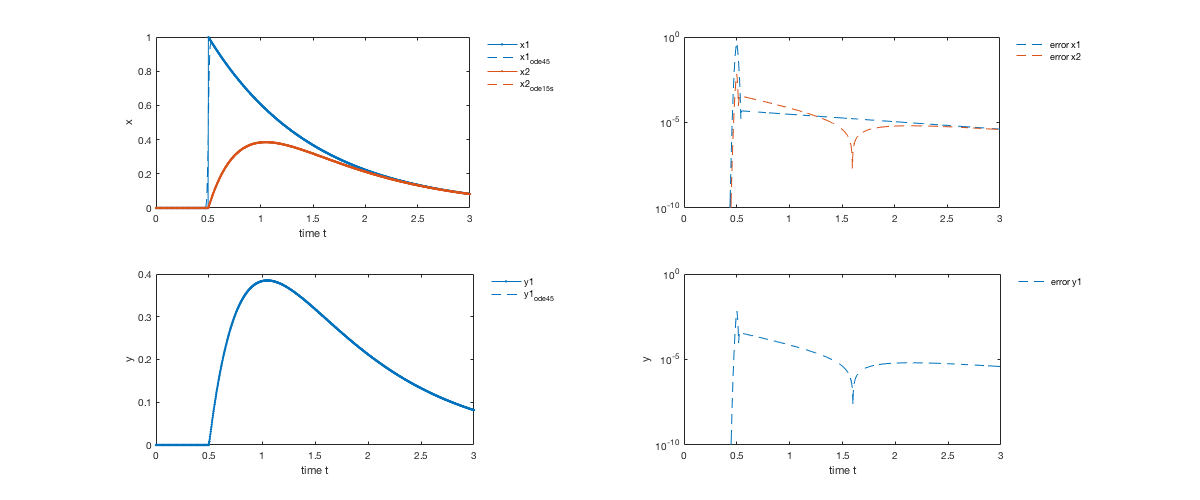
\includegraphics[width=\textwidth]{../../examples/example_dirac/html/example_dirac_01.png}
\begin{par}
FORWARD SENSITIVITY ANALYSIS
\end{par} \vspace{1em}
\begin{DoxyCode}
    options.sensi = 1;

    sol = simulate_model_dirac(t,log10(p),k,[],options);
\end{DoxyCode}
\begin{par}
FINITE DIFFERENCES
\end{par} \vspace{1em}
\begin{DoxyCode}
    eps = 1e-4;
    xi = log10(p);
    for ip = 1:4;
        xip = xi;
        xip(ip) = xip(ip) + eps;
        solp = simulate_model_dirac(t,xip,k,[],options);
        sx_fd(:,:,ip) = (solp.x - sol.x)/eps;
        sy_fd(:,:,ip) = (solp.y - sol.y)/eps;
    end
\end{DoxyCode}
\begin{par}
PLOTTING
\end{par} \vspace{1em}
\begin{DoxyCode}
    figure
    for ip = 1:4
        subplot(4,2,ip*2-1)
        hold on
        for ix = 1:size(sol.x,2)
            plot(t,sol.sx(:,ix,ip),'.-','Color',c_x(ix,:))
            plot(t,sx_fd(:,ix,ip),'--','Color',c_x(ix,:))
        end
        ylim([-2,2])
        legend('x1','x1_{fd}','x2','x2_{fd}','Location','NorthEastOutside')
        legend boxoff
        title(['state sensitivity for p' num2str(ip)])
        xlabel('time t')
        ylabel('x')
        box on

        subplot(4,2,ip*2)
        plot(t,abs(sol.sx(:,:,ip)-sx_fd(:,:,ip)),'r--')
        legend('error x1','error x2','Location','NorthEastOutside')
        legend boxoff
        title(['state sensitivity for p' num2str(ip)])
        xlabel('time t')
        ylabel('error')
        ylim([1e-12,1e0])
        set(gca,'YScale','log')
        box on
    end
    set(gcf,'Position',[100 300 1200 500])

    figure
    for ip = 1:4
        subplot(4,2,ip*2-1)
        hold on
        for iy = 1:size(sol.y,2)
            plot(t,sol.sy(:,iy,ip),'.-','Color',c_x(iy,:))
            plot(t,sy_fd(:,iy,ip),'--','Color',c_x(iy,:))
        end
        ylim([-2,2])
        legend('y1','y1_{fd}','Location','NorthEastOutside')
        legend boxoff
        title(['observable sensitivity for p' num2str(ip)])
        xlabel('time t')
        ylabel('y')
        box on

        subplot(4,2,ip*2)
        plot(t,abs(sol.sy(:,:,ip)-sy_fd(:,:,ip)),'r--')
        legend('error y1','Location','NorthEastOutside')
        legend boxoff
        title(['observable sensitivity for p' num2str(ip)])
        xlabel('time t')
        ylabel('error')
        ylim([1e-12,1e0])
        set(gca,'YScale','log')
        box on
    end
    set(gcf,'Position',[100 300 1200 500])

    drawnow
\end{DoxyCode}

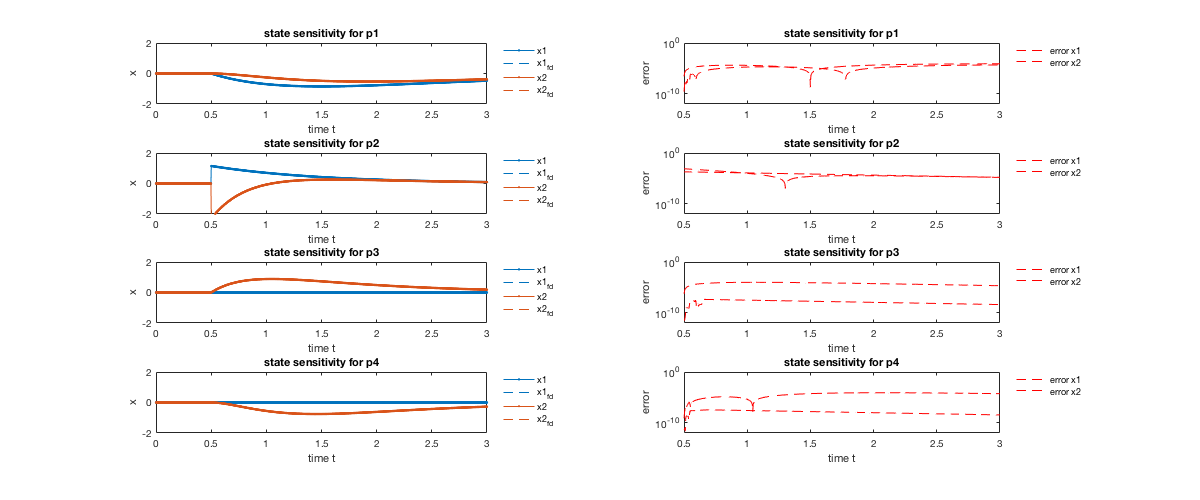
\includegraphics[width=\textwidth]{../../examples/example_dirac/html/example_dirac_02.png}

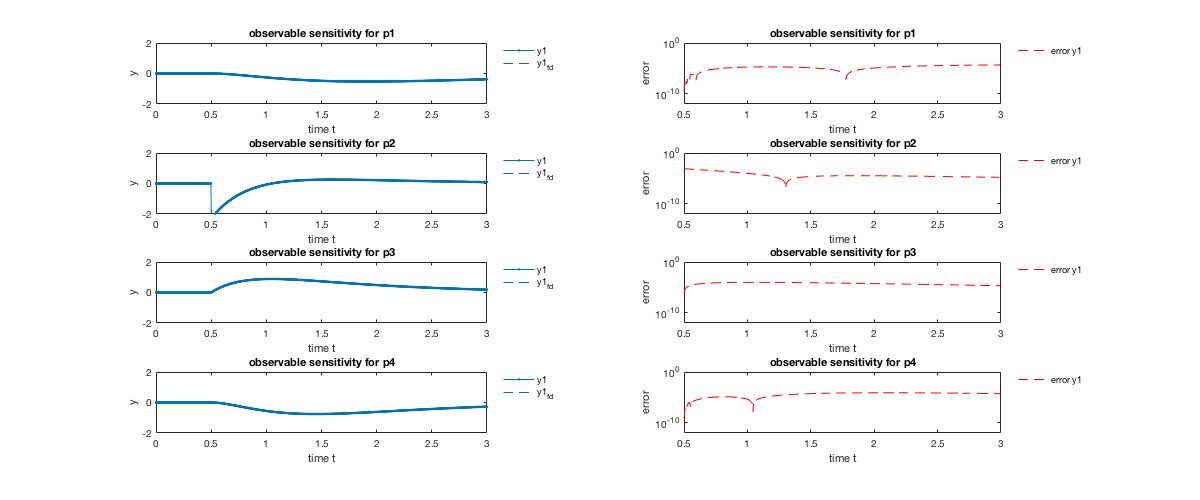
\includegraphics[width=\textwidth]{../../examples/example_dirac/html/example_dirac_03.png}
\begin{DoxyCode}
end
\end{DoxyCode}




     \hypertarget{example_steadystate}{}\subsection{Example Steady State}\label{example_steadystate}
\hypertarget{example_steadystate_def_steadystate}{}\subsubsection{Model Definition}\label{example_steadystate_def_steadystate}
 
% This LaTeX was auto-generated from MATLAB code.
% To make changes, update the MATLAB code and republish this document.











    
    \begin{DoxyCode}
function [model] = model_steadystate_syms()
\end{DoxyCode}
\begin{par}
STATES
\end{par} \vspace{1em}
\begin{DoxyCode}
% create state syms
syms x1 x2 x3

% create state vector
model.sym.x = [
x1 x2 x3
];
\end{DoxyCode}
\begin{par}
PARAMETERS ( for these sensitivities will be computed )
\end{par} \vspace{1em}
\begin{DoxyCode}
% create parameter syms
syms p1 p2 p3 p4 p5

% create parameter vector
model.sym.p = [p1,p2,p3,p4,p5];

% set the parametrisation of the problem options are 'log', 'log10' and
% 'lin' (default).
model.param = 'log10';
\end{DoxyCode}
\begin{par}
CONSTANTS ( for these no sensitivities will be computed ) this part is optional and can be ommited
\end{par} \vspace{1em}
\begin{DoxyCode}
% create parameter syms
syms k1 k2 k3 k4

% create parameter vector
model.sym.k = [k1 k2 k3 k4];
\end{DoxyCode}
\begin{par}
SYSTEM EQUATIONS
\end{par} \vspace{1em}
\begin{DoxyCode}
% create symbolic variable for time
syms t

model.sym.xdot = sym(zeros(size(model.sym.x)));

% piecewise defined function
model.sym.xdot(1) = -2*p1*x1^2 - p2*x1*x2 + 2*p3*x2 + p4*x3 + p5;
% inhomogeneous
model.sym.xdot(2) = +p1*x1^2 - p2*x1*x2 - p3*x2 + p4*x3;
model.sym.xdot(3) = p2*x1*x2 - p4*x3 - k4*x3;
\end{DoxyCode}
\begin{par}
INITIAL CONDITIONS
\end{par} \vspace{1em}
\begin{DoxyCode}
model.sym.x0 = sym(zeros(size(model.sym.x)));

model.sym.x0(1) = k1;
model.sym.x0(2) = k2;
model.sym.x0(3) = k3;
\end{DoxyCode}
\begin{par}
OBSERVALES
\end{par} \vspace{1em}
\begin{DoxyCode}
model.sym.y = model.sym.x;
\end{DoxyCode}
\begin{DoxyCode}
end
\end{DoxyCode}

         \begin{DoxyCode}ans = 
      sym: [1x1 struct]
    param: 'log10'
\end{DoxyCode} 
    



    \hypertarget{example_steadystate_simu_steadystate}{}\subsubsection{Simulation}\label{example_steadystate_simu_steadystate}
 
% This LaTeX was auto-generated from MATLAB code.
% To make changes, update the MATLAB code and republish this document.











    
    \begin{DoxyCode}
function example_steadystate
\end{DoxyCode}
\begin{par}
COMPILATION
\end{par} \vspace{1em}
\begin{DoxyCode}
    [exdir,~,~]=fileparts(which('example_steadystate.m'));
    % compile the model
    amiwrap('model_steadystate','model_steadystate_syms',exdir)
\end{DoxyCode}

         \begin{DoxyCode}Generating model struct ...
Parsing model struct ...

Generating C code ...
headers | wrapfunctions | 
Compiling mex file ...
amici | Building with 'Xcode with Clang'.
MEX completed successfully.
Building with 'Xcode with Clang'.
MEX completed successfully.
\end{DoxyCode} 
    \begin{par}
SIMULATION
\end{par} \vspace{1em}
\begin{DoxyCode}
    % time vector
    t = linspace(0,300,20);
    p = [1;0.5;0.4;2;0.1];
    k = [0.1,0.4,0.7,1];

    options = amioption('sensi',0,...
        'maxsteps',1e4);
    % load mex into memory
    sol = simulate_model_steadystate(t,log10(p),k,[],options);

    tic
    sol = simulate_model_steadystate(t,log10(p),k,[],options);
    disp(['Time elapsed with cvodes: ' num2str(toc) ])
\end{DoxyCode}

         \begin{DoxyCode}Time elapsed with cvodes: 0.004374
\end{DoxyCode} 
    \begin{par}
ODE15S
\end{par} \vspace{1em}
\begin{DoxyCode}
    ode_system = @(t,x,p,k) [-2*p(1)*x(1)^2 - p(2)*x(1)*x(2) + 2*p(3)*x(2) + p(4)*x(3) + p(5);
        + p(1)*x(1)^2 - p(2)*x(1)*x(2) - p(3)*x(2) + p(4)*x(3);
        + p(2)*x(1)*x(2) - p(4)*x(3) - k(4)*x(3)];
    options_ode15s = odeset('RelTol',options.rtol,'AbsTol',options.atol,'MaxStep',options.maxsteps);

    tic
    [~, X_ode15s] = ode15s(@(t,x) ode_system(t,x,p,k),t,k(1:3),options_ode15s);
    disp(['Time elapsed with ode15s: ' num2str(toc) ])
\end{DoxyCode}

         \begin{DoxyCode}Time elapsed with ode15s: 0.066508
\end{DoxyCode} 
    \begin{par}
PLOTTING
\end{par} \vspace{1em}
\begin{DoxyCode}
    figure
    c_x = get(gca,'ColorOrder');
    subplot(2,2,1)
    for ix = 1:size(sol.x,2)
        plot(t,sol.x(:,ix),'.-','Color',c_x(ix,:))
        hold on
        plot(t,X_ode15s(:,ix),'d','Color',c_x(ix,:))
    end
    legend('x1','x1_{ode15s}','x2','x2_{ode15s}','x3','x3_{ode15s}','Location','NorthEastOutside')
    legend boxoff
    xlabel('time t')
    ylabel('x')
    box on
    subplot(2,2,2)
    plot(t,abs(sol.x-X_ode15s),'--')
    set(gca,'YScale','log')
    legend('error x1','error x2','error x3','Location','NorthEastOutside')
    legend boxoff
    set(gcf,'Position',[100 300 1200 500])
\end{DoxyCode}

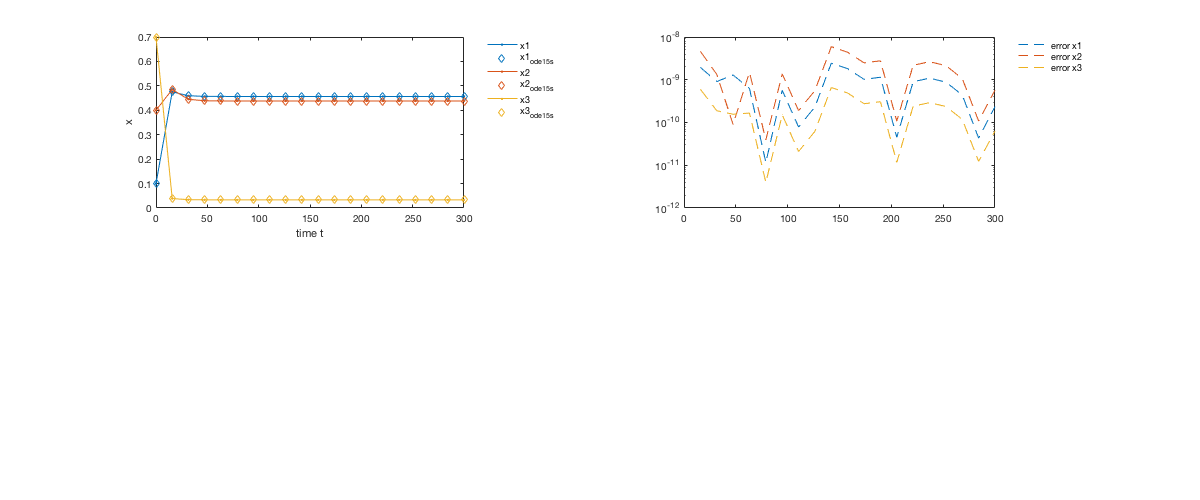
\includegraphics[width=\textwidth]{../../examples/example_steadystate/html/example_steadystate_01.png}
\begin{par}
FORWARD SENSITIVITY ANALYSIS
\end{par} \vspace{1em}
\begin{DoxyCode}
    options.sensi = 1;
    options.sens_ind = [3,1,2,4];

    sol = simulate_model_steadystate(t,log10(p),k,[],options);
\end{DoxyCode}
\begin{par}
FINITE DIFFERENCES
\end{par} \vspace{1em}
\begin{DoxyCode}
    eps = 1e-3;

    xi = log10(p);
    for ip = 1:4;
        xip = xi;
        xip(ip) = xip(ip) + eps;
        solp = simulate_model_steadystate(t,xip,k,[],options);
        sx_fd(:,:,ip) = (solp.x - sol.x)/eps;
        sy_fd(:,:,ip) = (solp.y - sol.y)/eps;
    end
\end{DoxyCode}
\begin{par}
PLOTTING
\end{par} \vspace{1em}
\begin{DoxyCode}
    figure
    for ip = 1:4
        subplot(4,2,ip*2-1)
        hold on
        for ix = 1:size(sol.x,2)
            plot(t,sol.sx(:,ix,ip),'.-','Color',c_x(ix,:))
            plot(t,sx_fd(:,ix,options.sens_ind(ip)),'d','Color',c_x(ix,:))
        end
        legend('x1','x1_{fd}','x2','x2_{fd}','x3','x3_{fd}','Location','NorthEastOutside')
        legend boxoff
        title(['state sensitivity for p' num2str(options.sens_ind(ip))])
        xlabel('time t')
        ylabel('x')
        box on

        subplot(4,2,ip*2)
        plot(t,abs(sol.sx(:,:,ip)-sx_fd(:,:,options.sens_ind(ip))),'--')
        legend('error x1','error x2','error x3','Location','NorthEastOutside')
        legend boxoff
        title(['error of state sensitivity for p' num2str(options.sens_ind(ip))])
        xlabel('time t')
        ylabel('error')
        set(gca,'YScale','log')
        box on
    end
    set(gcf,'Position',[100 300 1200 500])
\end{DoxyCode}

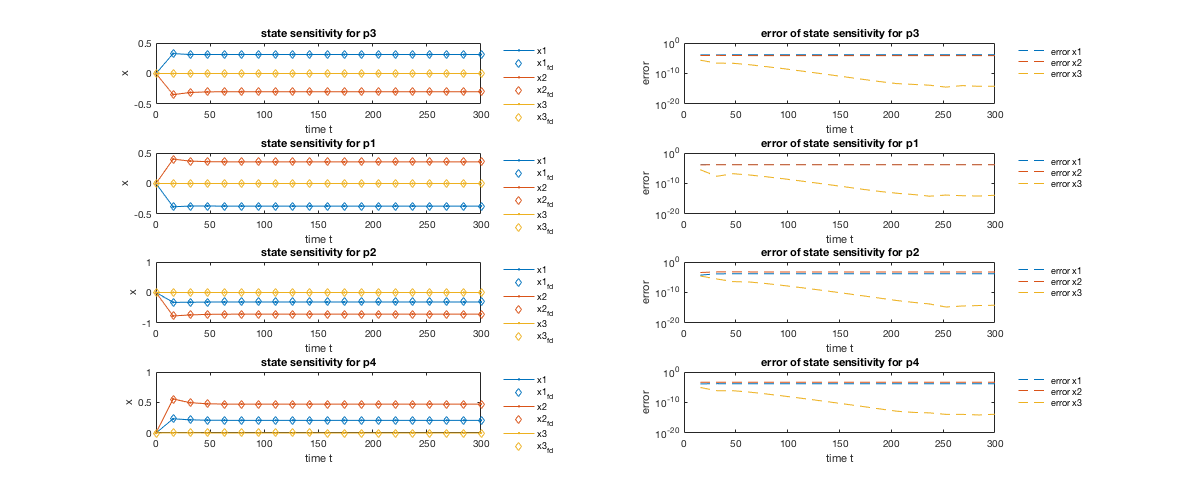
\includegraphics[width=\textwidth]{../../examples/example_steadystate/html/example_steadystate_02.png}
\begin{par}
STEADY STATE SENSITIVITY
\end{par} \vspace{1em}
\begin{DoxyCode}
    sssens = NaN(size(sol.sx));
    for it = 2:length(t)
        tt = [0,t(it)];
        options.sensi_meth = 'ss';
        solss = simulate_model_steadystate(tt,log10(p),k,[],options);
        sssens(it,:,:) = solss.sx;
        ssxdot(it,:) = solss.xdot;
    end
\end{DoxyCode}
\begin{par}
PLOTTING
\end{par} \vspace{1em}
\begin{DoxyCode}
    figure
    for ip = 1:4
        subplot(4,2,ip*2-1)
        hold on
        for ix = 1:size(sol.x,2)
            plot(t,sol.sx(:,ix,ip),'.-','Color',c_x(ix,:))
            plot(t,sssens(:,ix,ip),'d-','Color',c_x(ix,:))
        end
        legend('x1','x1_{ss}','x2','x2_{ss}','x3','x3_{ss}','Location','NorthEastOutside')
        legend boxoff
        title(['state steady sensitivity for p' num2str(ip)])
        xlabel('time t')
        ylabel('x')
        box on

        subplot(4,2,ip*2)
        plot(t,abs(sol.sx(:,:,ip)-sssens(:,:,ip)),'--')
        legend('error x1','error x2','error x3','Location','NorthEastOutside')
        legend boxoff
        title(['error of steady state sensitivity for p' num2str(ip)])
        xlabel('time t')
        ylabel('error')
        set(gca,'YScale','log')
        box on
    end
    set(gcf,'Position',[100 300 1200 500])

    figure
    scatter(sqrt(sum((ssxdot./sol.x).^2,2)),sqrt(sum(sum((sol.sx-sssens).^2,2),3)))
    hold on
    plot([1e-15,1e5],[1e-15,1e5],'k:')
    set(gca,'YScale','log')
    set(gca,'XScale','log')
    box on
    axis square
    xlabel('||dxdt/x||_2')
    ylabel('error steady state approximation')
    set(gca,'FontSize',15)
    set(gca,'LineWidth',1.5)
    set(gcf,'Position',[100 300 1200 500])

    drawnow
\end{DoxyCode}

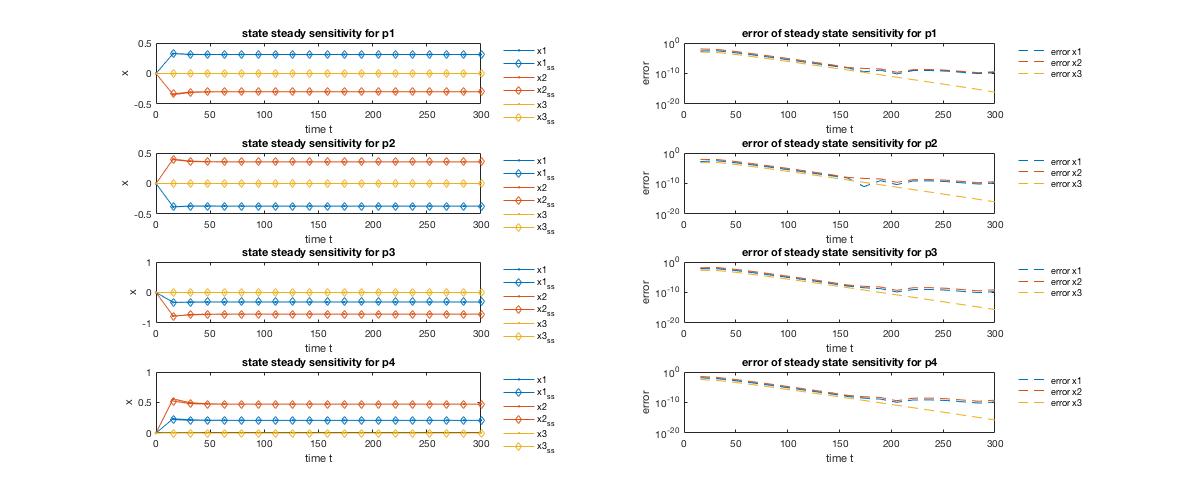
\includegraphics[width=\textwidth]{../../examples/example_steadystate/html/example_steadystate_03.png}

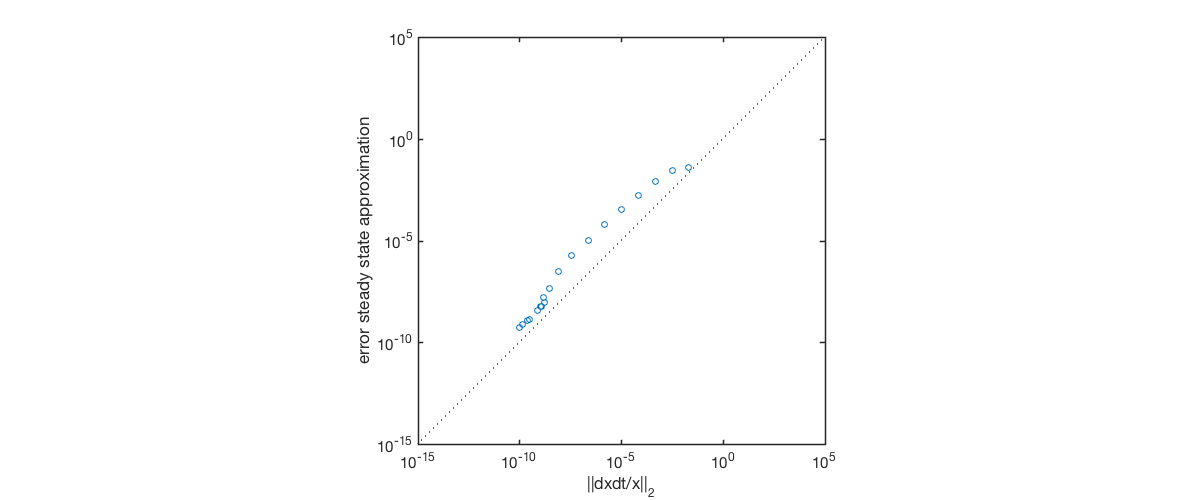
\includegraphics[width=\textwidth]{../../examples/example_steadystate/html/example_steadystate_04.png}
\begin{DoxyCode}
end
\end{DoxyCode}




     \hypertarget{example_jakstat_adjoint}{}\subsection{Example J\+A\+K/\+S\+T\+A\+T Adjoint}\label{example_jakstat_adjoint}
\hypertarget{example_jakstat_adjoint_def_jakstat_adjoint}{}\subsubsection{Model Definition}\label{example_jakstat_adjoint_def_jakstat_adjoint}
 
% This LaTeX was auto-generated from MATLAB code.
% To make changes, update the MATLAB code and republish this document.











    
    \begin{DoxyCode}
function [model] = model_jakstat_syms()
\end{DoxyCode}
\begin{par}
STATES
\end{par} \vspace{1em}
\begin{DoxyCode}
    syms STAT pSTAT pSTAT_pSTAT npSTAT_npSTAT nSTAT1 nSTAT2 nSTAT3 nSTAT4 nSTAT5

    model.sym.x = [
        STAT, pSTAT, pSTAT_pSTAT, npSTAT_npSTAT, nSTAT1, nSTAT2, nSTAT3, nSTAT4, nSTAT5 ...
        ];
\end{DoxyCode}
\begin{par}
PARAMETERS
\end{par} \vspace{1em}
\begin{DoxyCode}
    syms p1 p2 p3 p4 init_STAT Omega_cyt Omega_nuc sp1 sp2 sp3 sp4 sp5 offset_tSTAT offset_pSTAT scale_tSTAT scale_pSTAT sigma_pSTAT sigma_tSTAT sigma_pEpoR

    model.sym.p = [p1,p2,p3,p4,init_STAT,sp1,sp2,sp3,sp4,sp5,offset_tSTAT,offset_pSTAT,scale_tSTAT,scale_pSTAT,sigma_pSTAT,sigma_tSTAT,sigma_pEpoR];

    model.param = 'log10';

    model.sym.k = [Omega_cyt,Omega_nuc];
\end{DoxyCode}
\begin{par}
INPUT
\end{par} \vspace{1em}
\begin{DoxyCode}
    syms t
    u(1) = spline_pos5(t, 0.0, sp1, 5.0, sp2, 10.0, sp3, 20.0, sp4, 60.0, sp5, 0, 0.0);
\end{DoxyCode}

         \begin{DoxyCode}Warning: Support of strings that are not valid variable names or define a number
will be removed in a future release. To create symbolic expressions, first
create symbolic variables and then use operations on them. 
\end{DoxyCode} 
    \begin{par}
SYSTEM EQUATIONS
\end{par} \vspace{1em}
\begin{DoxyCode}
    model.sym.xdot = sym(zeros(size(model.sym.x)));

    model.sym.xdot(1) = (Omega_nuc*p4*nSTAT5 - Omega_cyt*STAT*p1*u(1))/Omega_cyt;
    model.sym.xdot(2) = STAT*p1*u(1) - 2*p2*pSTAT^2;
    model.sym.xdot(3) = p2*pSTAT^2 - p3*pSTAT_pSTAT;
    model.sym.xdot(4) = -(Omega_nuc*p4*npSTAT_npSTAT - Omega_cyt*p3*pSTAT_pSTAT)/Omega_nuc;
    model.sym.xdot(5) = -p4*(nSTAT1 - 2*npSTAT_npSTAT);
    model.sym.xdot(6) = p4*(nSTAT1 - nSTAT2);
    model.sym.xdot(7) = p4*(nSTAT2 - nSTAT3);
    model.sym.xdot(8) = p4*(nSTAT3 - nSTAT4);
    model.sym.xdot(9) = p4*(nSTAT4 - nSTAT5);
\end{DoxyCode}
\begin{par}
INITIAL CONDITIONS
\end{par} \vspace{1em}
\begin{DoxyCode}
    model.sym.x0 = sym(zeros(size(model.sym.x)));

    model.sym.x0(1) = init_STAT;
\end{DoxyCode}
\begin{par}
OBSERVABLES
\end{par} \vspace{1em}
\begin{DoxyCode}
    model.sym.y = sym(zeros(3,1));

    model.sym.y(1) = offset_pSTAT + scale_pSTAT/init_STAT*(pSTAT + 2*pSTAT_pSTAT);
    model.sym.y(2) = offset_tSTAT + scale_tSTAT/init_STAT*(STAT + pSTAT + 2*(pSTAT_pSTAT));
    model.sym.y(3) = u(1);
\end{DoxyCode}
\begin{par}
SIGMA
\end{par} \vspace{1em}
\begin{DoxyCode}
    model.sym.sigma_y = sym(size(model.sym.y));

    model.sym.sigma_y(1) = sigma_pSTAT;
    model.sym.sigma_y(2) = sigma_tSTAT;
    model.sym.sigma_y(3) = sigma_pEpoR;
\end{DoxyCode}
\begin{DoxyCode}
end
\end{DoxyCode}

         \begin{DoxyCode}ans = 
      sym: [1x1 struct]
    param: 'log10'
\end{DoxyCode} 
    



    \hypertarget{example_jakstat_adjoint_simu_jakstat_adjoint}{}\subsubsection{Simulation}\label{example_jakstat_adjoint_simu_jakstat_adjoint}
 
% This LaTeX was auto-generated from MATLAB code.
% To make changes, update the MATLAB code and republish this document.











    
    \begin{DoxyCode}
function example_jakstat_adjoint()

    % compile the model
    [exdir,~,~]=fileparts(which('example_jakstat_adjoint.m'));
    amiwrap('model_jakstat','model_jakstat_adjoint_syms',exdir)

    num = xlsread(fullfile(exdir,'pnas_data_original.xls'));

    D.t = num(:,1);
    D.condition= [1.4,0.45];
    D.Y = num(:,[2,4,6]);
    D.Sigma_Y = NaN(size(D.Y));
    D = amidata(D);

    xi =  [0.60
        3
        -0.95
        -0.0075
        0
        -2.8
        -0.26
        -0.075
        -0.41
        -5
        -0.74
        -0.64
        -0.11
        0.027
        -0.5
        0
        -0.5];

    options.sensi = 0;
    sol = simulate_model_jakstat([],xi,[],D,options);

    figure
    for iy = 1:3
        subplot(2,2,iy)
        plot(D.t,D.Y(:,iy),'rx')
        hold on
        plot(sol.t,sol.y(:,iy),'.-')
        xlim([0,60])
        xlabel('t')
        switch(iy)
            case 1
                ylabel('pStat')
            case 2
                ylabel('tStat')
            case 3
                ylabel('pEpoR')
        end
        ylim([0,1.2])
    end
    set(gcf,'Position',[100 300 1200 500])

    % generate new
    xi_rand = xi + 0.1;
    options.sensi = 1;
    options.sensi_meth = 'adjoint';
    sol = simulate_model_jakstat([],xi_rand,[],D,options);

    options.sensi = 0;
    eps = 1e-4;
    fd_grad = NaN(length(xi),1);
    for ip = 1:length(xi)
        xip = xi_rand;
        xip(ip) = xip(ip) + eps;
        psol = simulate_model_jakstat([],xip,[],D,options);
        fd_grad(ip) = (psol.llh-sol.llh)/eps;
    end

    figure
    scatter(abs(sol.sllh),abs(fd_grad))
    set(gca,'XScale','log')
    set(gca,'YScale','log')
    xlim([1e-2,1e2])
    ylim([1e-2,1e2])
    box on
    hold on
    axis square
    plot([1e-2,1e2],[1e-2,1e2],'k:')
    xlabel('adjoint sensitivity absolute value of gradient element')
    ylabel('finite difference absolute value of gradient element')
    set(gcf,'Position',[100 300 1200 500])


    drawnow

end
\end{DoxyCode}

         \begin{DoxyCode}Generating model struct ...
Parsing model struct ...

Generating C code ...
headers | wrapfunctions | 
Compiling mex file ...
amici | Building with 'Xcode with Clang'.
MEX completed successfully.
Building with 'Xcode with Clang'.
MEX completed successfully.
\end{DoxyCode} 
    
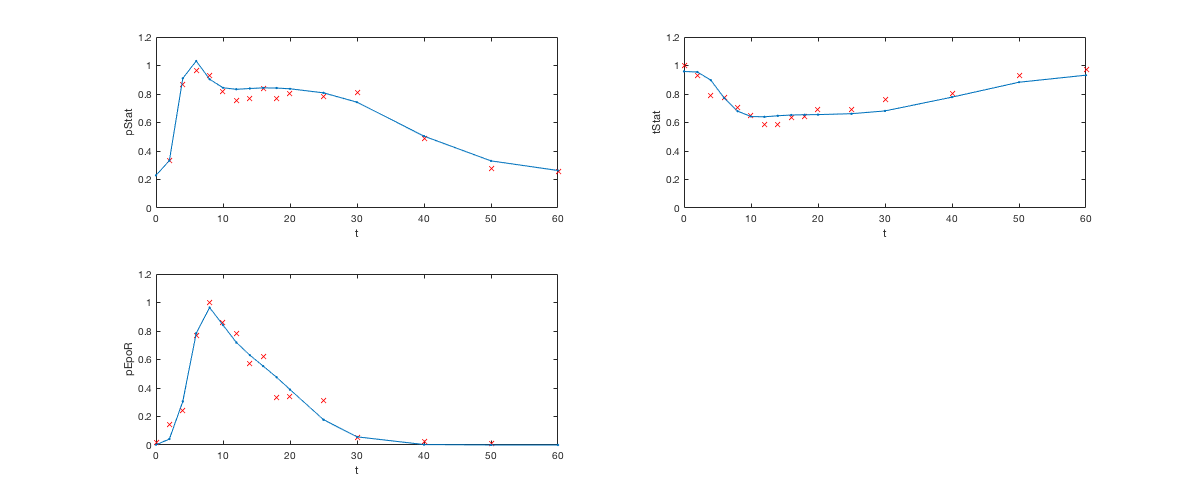
\includegraphics[width=\textwidth]{../../examples/example_jakstat_adjoint/html/example_jakstat_adjoint_01.png}

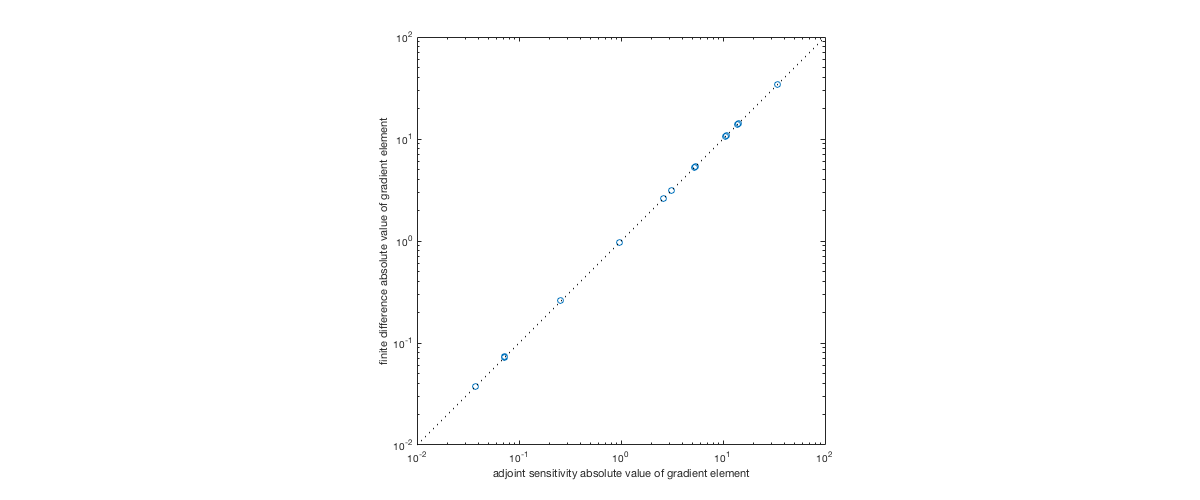
\includegraphics[width=\textwidth]{../../examples/example_jakstat_adjoint/html/example_jakstat_adjoint_02.png}




     \hypertarget{example_dirac_adjoint}{}\subsection{Example Dirac Adjoint}\label{example_dirac_adjoint}
\hypertarget{example_dirac_adjoint_def_dirac_adjoint}{}\subsubsection{Model Definition}\label{example_dirac_adjoint_def_dirac_adjoint}
 
% This LaTeX was auto-generated from MATLAB code.
% To make changes, update the MATLAB code and republish this document.











    
    \begin{DoxyCode}
function [model] = model_dirac_adjoint_syms()
\end{DoxyCode}
\begin{par}
STATES
\end{par} \vspace{1em}
\begin{DoxyCode}
% create state syms
syms x1 x2

% create state vector
model.sym.x = [ x1 x2 ];
\end{DoxyCode}
\begin{par}
PARAMETERS ( for these sensitivities will be computed )
\end{par} \vspace{1em}
\begin{DoxyCode}
% create parameter syms
syms p1 p2 p3 p4

% create parameter vector
model.sym.p = [p1,p2,p3,p4];

% set the parametrisation of the problem options are 'log', 'log10' and
% 'lin' (default).
model.param = 'log10';
\end{DoxyCode}
\begin{par}
SYSTEM EQUATIONS
\end{par} \vspace{1em}
\begin{DoxyCode}
% create symbolic variable for time
syms t

model.sym.xdot = sym(zeros(size(model.sym.x)));

% piecewise defined function
model.sym.xdot(1) = -p1*x1 + dirac(t-p2);
% inhomogeneous
model.sym.xdot(2) = p3*x1 - p4*x2 ;
\end{DoxyCode}
\begin{par}
INITIAL CONDITIONS
\end{par} \vspace{1em}
\begin{DoxyCode}
model.sym.x0 = sym(zeros(size(model.sym.x)));

model.sym.x0(1) = 0;
model.sym.x0(2) = 0;
\end{DoxyCode}
\begin{par}
OBSERVALES
\end{par} \vspace{1em}
\begin{DoxyCode}
model.sym.y = sym(zeros(1,1));

model.sym.y(1) = x2;
\end{DoxyCode}
\begin{DoxyCode}
end
\end{DoxyCode}

         \begin{DoxyCode}ans = 
      sym: [1x1 struct]
    param: 'log10'
\end{DoxyCode} 
    



    \hypertarget{example_dirac_adjoint_simu_dirac_adjoint}{}\subsubsection{Simulation}\label{example_dirac_adjoint_simu_dirac_adjoint}
 
% This LaTeX was auto-generated from MATLAB code.
% To make changes, update the MATLAB code and republish this document.











    
    \begin{DoxyCode}
function example_dirac_adjoint()
\end{DoxyCode}
\begin{par}
COMPILATION
\end{par} \vspace{1em}
\begin{DoxyCode}
    [exdir,~,~]=fileparts(which('example_dirac_adjoint.m'));
    % compile the model
    amiwrap('model_dirac_adjoint','model_dirac_adjoint_syms',exdir)
\end{DoxyCode}

         \begin{DoxyCode}Generating model struct ...
Parsing model struct ...

Generating C code ...
headers | wrapfunctions | 
Compiling mex file ...
amici | Building with 'Xcode with Clang'.
MEX completed successfully.
Building with 'Xcode with Clang'.
MEX completed successfully.
\end{DoxyCode} 
    \begin{par}
SIMULATION
\end{par} \vspace{1em}
\begin{DoxyCode}
    % time vector
    tout = linspace(0,4,9);
    tfine = linspace(0,4,10001);
    p = [1;0.4;2;3];
    k = [];

    D.Y = [  0.00714742903826096
        -0.00204966058299775
        0.382159034587845
        0.33298932672138
        0.226111476113441
        0.147028440865854
        0.0882468698791813
        0.0375887796628869
        0.0373422340295005];

    D.Sigma_Y = 0.01*ones(size(D.Y));


    options.sensi = 1;
    options.sensi_meth = 'adjoint';
    options.maxsteps = 1e5;
    sol = simulate_model_dirac_adjoint(tout,log10(p),k,D,options);
    options.sensi = 0;
    solfine = simulate_model_dirac_adjoint(tfine,log10(p),k,[],options);
    figure
    errorbar(tout,D.Y,D.Sigma_Y)
    hold on
    plot(tfine,solfine.y)
    legend('data','simulation')
    xlabel('time t')
    ylabel('observable')
    title(['log-likelihood: ' num2str(sol.llh) ])
\end{DoxyCode}

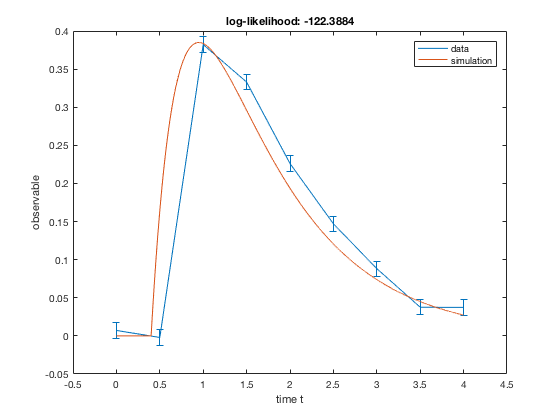
\includegraphics[width=\textwidth]{../../examples/example_dirac_adjoint/html/example_dirac_adjoint_01.png}
\begin{par}
FD
\end{par} \vspace{1em}
\begin{DoxyCode}
    eps = 1e-4;
    xi = log10(p);
    grad_fd_f = NaN(4,1);
    grad_fd_b = NaN(4,1);
    for ip = 1:4;
        options.sensi = 0;
        xip = xi;
        xip(ip) = xip(ip) + eps;
        solpf = simulate_model_dirac_adjoint(tout,xip,k,D,options);
        grad_fd_f(ip,1) = (solpf.llh-sol.llh)/eps;
        xip = xi;
        xip(ip) = xip(ip) - eps;
        solpb = simulate_model_dirac_adjoint(tout,xip,k,D,options);
        grad_fd_b(ip,1) = -(solpb.llh-sol.llh)/eps;
    end

    figure
    plot(abs(grad_fd_f),abs(sol.sllh),'o')
    hold on
    plot(abs(grad_fd_b),abs(sol.sllh),'o')
    set(gca,'XScale','log')
    set(gca,'YScale','log')
    hold on
    axis square
    plot([1e2,1e4],[1e2,1e4],'k:')
    xlim([1e2,1e4])
    ylim([1e2,1e4])
    legend('forward FD','backward FD','Location','SouthEast')
    xlabel('adjoint sensitivity absolute value of gradient element')
    ylabel('computed absolute value of gradient element')
    set(gcf,'Position',[100 300 1200 500])

    drawnow
\end{DoxyCode}

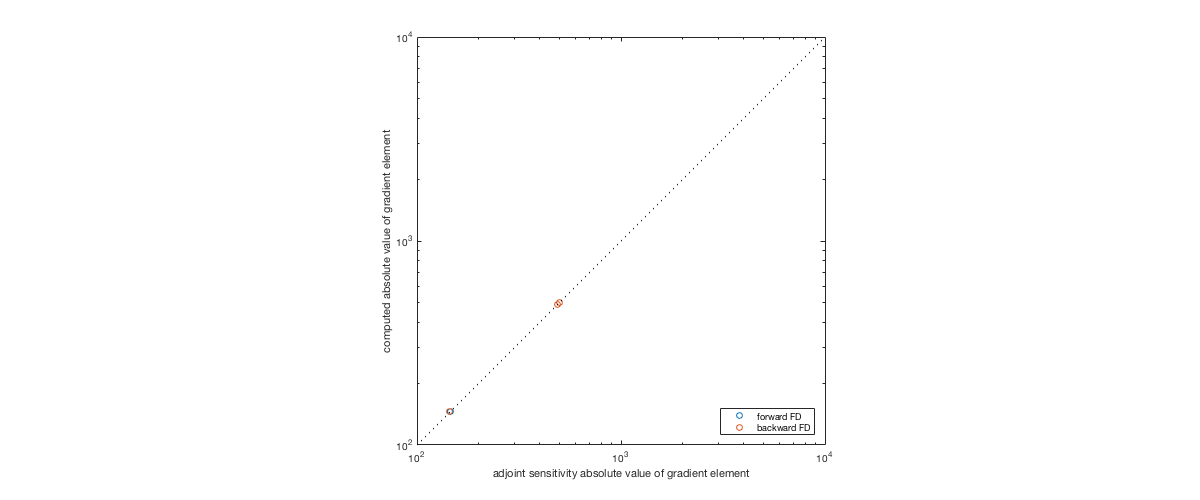
\includegraphics[width=\textwidth]{../../examples/example_dirac_adjoint/html/example_dirac_adjoint_02.png}
\begin{DoxyCode}
end
\end{DoxyCode}




     \hypertarget{example_dirac_secondorder}{}\subsection{Example Dirac Second Order Forward}\label{example_dirac_secondorder}
\hypertarget{example_dirac_secondorder_def_dirac_secondorder}{}\subsubsection{Model Definition}\label{example_dirac_secondorder_def_dirac_secondorder}
 
% This LaTeX was auto-generated from MATLAB code.
% To make changes, update the MATLAB code and republish this document.











    
    \begin{DoxyCode}
function [model] = model_dirac_secondorder_syms()
\end{DoxyCode}
\begin{par}
STATES
\end{par} \vspace{1em}
\begin{DoxyCode}
% create state syms
syms x1 x2

% create state vector
model.sym.x = [ x1 x2 ];
\end{DoxyCode}
\begin{par}
PARAMETERS ( for these sensitivities will be computed )
\end{par} \vspace{1em}
\begin{DoxyCode}
% create parameter syms
syms p1 p2 p3 p4

% create parameter vector
model.sym.p = [p1,p2,p3,p4];

% set the parametrisation of the problem options are 'log', 'log10' and
% 'lin' (default).
model.param = 'log10';
\end{DoxyCode}
\begin{par}
SYSTEM EQUATIONS
\end{par} \vspace{1em}
\begin{DoxyCode}
% create symbolic variable for time
syms t

model.sym.xdot = sym(zeros(size(model.sym.x)));

% piecewise defined function
model.sym.xdot(1) = -p1*x1 + dirac(t-p2);
% inhomogeneous
model.sym.xdot(2) = p3*x1 - p4*x2 ;
\end{DoxyCode}
\begin{par}
INITIAL CONDITIONS
\end{par} \vspace{1em}
\begin{DoxyCode}
model.sym.x0 = sym(zeros(size(model.sym.x)));

model.sym.x0(1) = 0;
model.sym.x0(2) = 0;
\end{DoxyCode}
\begin{par}
OBSERVALES
\end{par} \vspace{1em}
\begin{DoxyCode}
model.sym.y = sym(zeros(1,1));

model.sym.y(1) = x2;
\end{DoxyCode}
\begin{DoxyCode}
end
\end{DoxyCode}

         \begin{DoxyCode}ans = 
      sym: [1x1 struct]
    param: 'log10'
\end{DoxyCode} 
    



    \hypertarget{example_dirac_secondorder_simu_dirac_secondorder}{}\subsubsection{Simulation}\label{example_dirac_secondorder_simu_dirac_secondorder}
 
% This LaTeX was auto-generated from MATLAB code.
% To make changes, update the MATLAB code and republish this document.











    
    \begin{DoxyCode}
function example_dirac_secondorder()
\end{DoxyCode}
\begin{par}
COMPILATION
\end{par} \vspace{1em}
\begin{DoxyCode}
    [exdir,~,~]=fileparts(which('example_dirac_secondorder.m'));
    % compile the model
    amiwrap('model_dirac_secondorder','model_dirac_secondorder_syms',exdir,1)
\end{DoxyCode}

         \begin{DoxyCode}Generating model struct ...
x | k | p | deltax | xdot | deltaxdot | ddeltaxdx | ddeltaxdp | ddeltaxdt | root | drootdx | sx | drootdp | drootdt | dtaudp | sroot | stau | deltasx | sigma_y | dsigma_ydp | y | dydp | sigma_z | dsigma_zdp | z | dzdp | Parsing model struct ...
z | 

Generating C code ...
deltasx | deltax | dsigma_ydp | dsigma_zdp | dydp | dzdp | root | sigma_y | sigma_z | stau | xdot | y | z | headers | wrapfunctions | 
headers | wrapfunctions | 
Compiling mex file ...
amici | Building with 'Xcode with Clang'.
MEX completed successfully.
Building with 'Xcode with Clang'.
MEX completed successfully.
amici | Building with 'Xcode with Clang'.
MEX completed successfully.
Building with 'Xcode with Clang'.
MEX completed successfully.
\end{DoxyCode} 
    \begin{par}
SIMULATION
\end{par} \vspace{1em}
\begin{DoxyCode}
    % time vector
    t = linspace(0,3,1001);
    p = [1;0.5;2;3];
    k = [];

    options = amioption('sensi',0,...
        'maxsteps',1e4);

    % load mex into memory
    [msg] = which('simulate_model_secondorder_dirac'); % fix for inaccessability problems
    options.sensi = 2;
    sol = simulate_model_dirac_secondorder(t,log10(p),k,[],options);
\end{DoxyCode}
\begin{par}
FORWARD SENSITIVITY ANALYSIS
\end{par} \vspace{1em}
\begin{DoxyCode}
    options.sensi = 2;

    sol = simulate_model_dirac_secondorder(t,log10(p),k,[],options);
\end{DoxyCode}
\begin{par}
FINITE DIFFERENCES
\end{par} \vspace{1em}
\begin{DoxyCode}
    options.sensi = 1;

    eps = 1e-4;
    xi = log10(p);
    for ip = 1:4;
        xip = xi;
        xip(ip) = xip(ip) + eps;
        solp = simulate_model_dirac_secondorder(t,xip,k,[],options);
        s2x_fd(:,:,:,ip) = (solp.sx - sol.sx)/eps;
        s2y_fd(:,:,:,ip) = (solp.sy - sol.sy)/eps;
    end
\end{DoxyCode}
\begin{par}
PLOTTING
\end{par} \vspace{1em}
\begin{DoxyCode}
    figure
    c_x = get(gca,'ColorOrder');
    for ip = 1:4
        for jp = 1:4
            subplot(4,4,(ip-1)*4+jp)
            hold on
            for ix = 1:size(sol.x,2)
                plot(t,sol.s2x(:,ix,ip,jp),'.-','Color',c_x(ix,:))
                plot(t,s2x_fd(:,ix,ip,jp),'--','Color',c_x(ix,:))
            end
            ylim([-10,10])
            legend('x1','x1_{fd}','x2','x2_{fd}','Location','NorthEastOutside')
            legend boxoff
            title(['state sensitivity for p' num2str(ip) '/p' num2str(jp)])
            xlabel('time t')
            ylabel('x')
            box on
        end
    end
    set(gcf,'Position',[100 300 1200 500])
    figure
    for ip = 1:4
        for jp = 1:4
            subplot(4,4,(ip-1)*4+jp)
            plot(t,abs(sol.s2x(:,:,ip,jp)-s2x_fd(:,:,ip,jp)),'r--')
            legend('error x1','error x2','Location','NorthEastOutside')
            legend boxoff
            title(['state sensitivity for p' num2str(ip) '/p' num2str(jp)])
            xlabel('time t')
            ylabel('error')
            ylim([1e-12,1e0])
            set(gca,'YScale','log')
            box on
        end
    end
    set(gcf,'Position',[100 300 1200 500])

    drawnow
\end{DoxyCode}

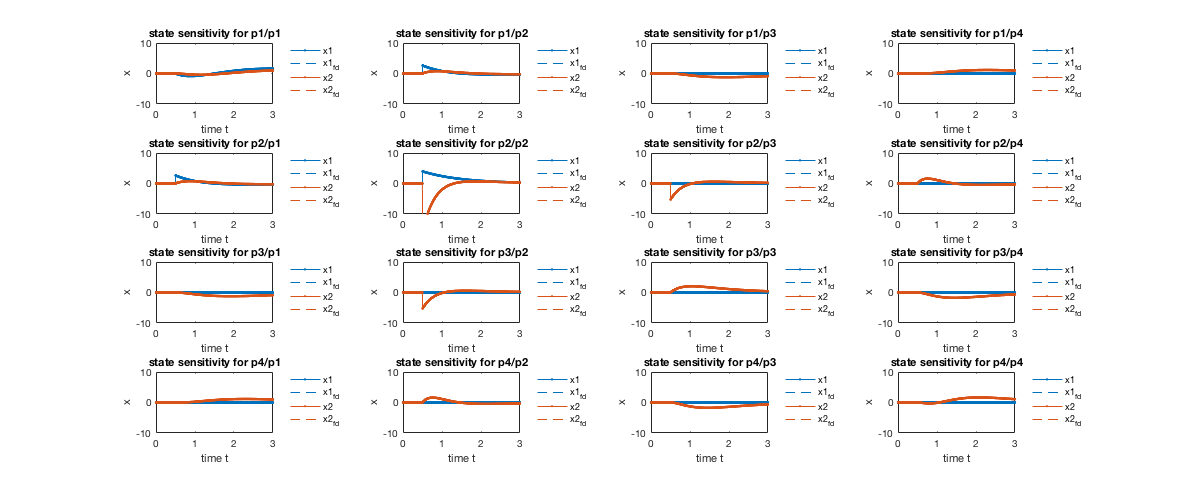
\includegraphics[width=\textwidth]{../../examples/example_dirac_secondorder/html/example_dirac_secondorder_01.png}

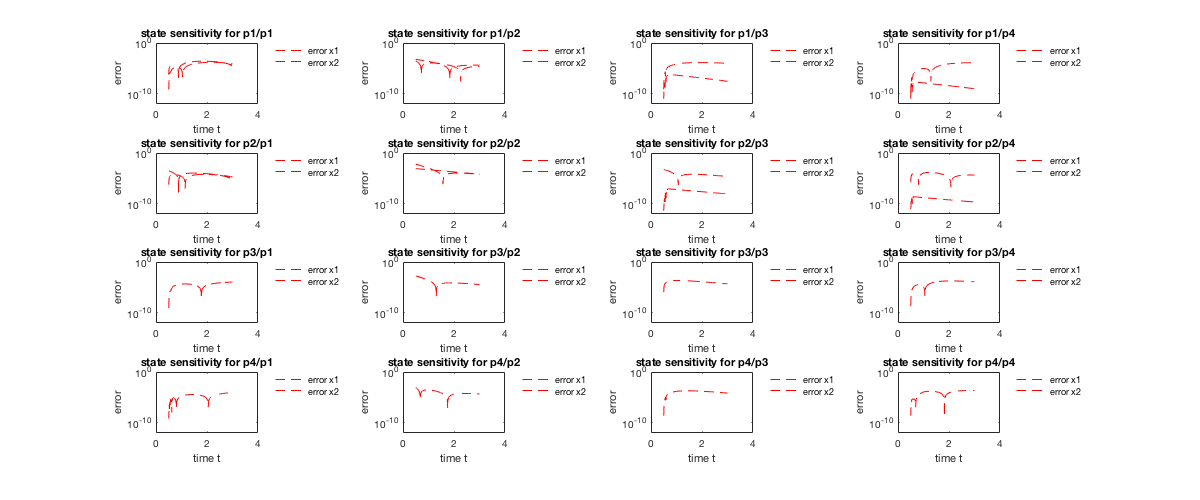
\includegraphics[width=\textwidth]{../../examples/example_dirac_secondorder/html/example_dirac_secondorder_02.png}
\begin{DoxyCode}
end
\end{DoxyCode}




     \hypertarget{example_dirac_secondorder_vectmult}{}\subsection{Example Dirac Directional Second Order Forward}\label{example_dirac_secondorder_vectmult}
\hypertarget{example_dirac_secondorder_vectmult_def_dirac_secondorder_vectmult}{}\subsubsection{Model Definition}\label{example_dirac_secondorder_vectmult_def_dirac_secondorder_vectmult}
 
% This LaTeX was auto-generated from MATLAB code.
% To make changes, update the MATLAB code and republish this document.











    
    \begin{DoxyCode}
function [model] = model_dirac_secondorder_vectmult_syms()
\end{DoxyCode}
\begin{par}
STATES
\end{par} \vspace{1em}
\begin{DoxyCode}
% create state syms
syms x1 x2

% create state vector
model.sym.x = [ x1 x2 ];
\end{DoxyCode}
\begin{par}
PARAMETERS ( for these sensitivities will be computed )
\end{par} \vspace{1em}
\begin{DoxyCode}
% create parameter syms
syms p1 p2 p3 p4

% create parameter vector
model.sym.p = [p1,p2,p3,p4];

% set the parametrisation of the problem options are 'log', 'log10' and
% 'lin' (default).
model.param = 'log10';
\end{DoxyCode}
\begin{par}
SYSTEM EQUATIONS
\end{par} \vspace{1em}
\begin{DoxyCode}
% create symbolic variable for time
syms t

model.sym.xdot = sym(zeros(size(model.sym.x)));

% piecewise defined function
model.sym.xdot(1) = -p1*x1 + dirac(t-p2);
% inhomogeneous
model.sym.xdot(2) = p3*x1 - p4*x2 ;
\end{DoxyCode}
\begin{par}
INITIAL CONDITIONS
\end{par} \vspace{1em}
\begin{DoxyCode}
model.sym.x0 = sym(zeros(size(model.sym.x)));

model.sym.x0(1) = 0;
model.sym.x0(2) = 0;
\end{DoxyCode}
\begin{par}
OBSERVALES
\end{par} \vspace{1em}
\begin{DoxyCode}
model.sym.y = sym(zeros(1,1));

model.sym.y(1) = x2;
\end{DoxyCode}
\begin{DoxyCode}
end
\end{DoxyCode}

         \begin{DoxyCode}ans = 
      sym: [1x1 struct]
    param: 'log10'
\end{DoxyCode} 
    



    \hypertarget{example_dirac_secondorder_vectmult_simu_dirac_secondorder_vectmult}{}\subsubsection{Simulation}\label{example_dirac_secondorder_vectmult_simu_dirac_secondorder_vectmult}
 
% This LaTeX was auto-generated from MATLAB code.
% To make changes, update the MATLAB code and republish this document.











    
    \begin{DoxyCode}
function example_dirac_secondorder_vectmult()
\end{DoxyCode}
\begin{par}
COMPILATION
\end{par} \vspace{1em}
\begin{DoxyCode}
    [exdir,~,~]=fileparts(which('example_dirac_secondorder_vectmult.m'));
    % compile the model
    amiwrap('model_dirac_secondorder_vectmult','model_dirac_secondorder_vectmult_syms',exdir,2)
\end{DoxyCode}

         \begin{DoxyCode}Generating model struct ...
x | k | p | deltax | xdot | deltaxdot | ddeltaxdx | ddeltaxdp | ddeltaxdt | root | drootdx | sx | drootdp | drootdt | dtaudp | sroot | stau | deltasx | sigma_y | dsigma_ydp | y | dydp | sigma_z | dsigma_zdp | z | dzdp | Parsing model struct ...
z | 

Generating C code ...
deltasx | deltax | dsigma_ydp | dsigma_zdp | dydp | dzdp | root | sigma_y | sigma_z | stau | xdot | y | z | headers | wrapfunctions | 
headers | wrapfunctions | 
Compiling mex file ...
amici | Building with 'Xcode with Clang'.
MEX completed successfully.
Building with 'Xcode with Clang'.
MEX completed successfully.
amici | Building with 'Xcode with Clang'.
MEX completed successfully.
Building with 'Xcode with Clang'.
MEX completed successfully.
\end{DoxyCode} 
    \begin{par}
SIMULATION
\end{par} \vspace{1em}
\begin{DoxyCode}
    % time vector
    t = linspace(0,3,1001);
    p = [1;0.5;2;3];
    k = [];
    v = [0.7;0.3;1.4;0.1];

    options = amioption('sensi',0,...
        'maxsteps',1e4);

    % load mex into memory
    [msg] = which('model_dirac_secondorder_vectmult'); % fix for inaccessability problems
    options.sensi = 2;
    sol = simulate_model_dirac_secondorder_vectmult(t,log10(p),k,[],options,v);
\end{DoxyCode}
\begin{par}
FORWARD SENSITIVITY ANALYSIS
\end{par} \vspace{1em}
\begin{DoxyCode}
    options.sensi = 2;

    sol = simulate_model_dirac_secondorder_vectmult(t,log10(p),k,[],options,v);
\end{DoxyCode}
\begin{par}
FINITE DIFFERENCES
\end{par} \vspace{1em}
\begin{DoxyCode}
    options.sensi = 1;

    eps = 1e-4;
    xi = log10(p);
    for ip = 1:4;
        xip = xi;
        xip(ip) = xip(ip) + eps;
        solp = simulate_model_dirac_secondorder_vectmult(t,xip,k,[],options);
        s2x_fd(:,:,ip) = sum(bsxfun(@times,(solp.sx - sol.sx)/eps,permute(v,[3,2,1])),3);
        s2y_fd(:,:,ip) = sum(bsxfun(@times,(solp.sy - sol.sy)/eps,permute(v,[3,2,1])),3);
    end
\end{DoxyCode}
\begin{par}
PLOTTING
\end{par} \vspace{1em}
\begin{DoxyCode}
    figure
    c_x = get(gca,'ColorOrder');
    for ip = 1:4
        subplot(4,2,ip*2-1)
        hold on
        for ix = 1:size(sol.x,2)
            plot(t,sol.s2x(:,ix,ip),'.-','Color',c_x(ix,:))
            plot(t,s2x_fd(:,ix,ip),'--','Color',c_x(ix,:))
        end
        ylim([-10,10])
        legend('x1','x1_{fd}','x2','x2_{fd}','Location','NorthEastOutside')
        legend boxoff
        title(['state sensitivity for p' num2str(ip)])
        xlabel('time t')
        ylabel('x')
        box on

        subplot(4,2,ip*2)
        plot(t,abs(sol.s2x(:,:,ip)-s2x_fd(:,:,ip)),'r--')
        legend('error x1','error x2','Location','NorthEastOutside')
        legend boxoff
        title(['state sensitivity for p' num2str(ip)])
        xlabel('time t')
        ylabel('error')
        ylim([1e-12,1e0])
        set(gca,'YScale','log')
        box on
    end
    set(gcf,'Position',[100 300 1200 500])

    figure
    for ip = 1:4
        subplot(4,2,ip*2-1)
        hold on
        for iy = 1:size(sol.y,2)
            plot(t,sol.s2y(:,iy,ip),'.-','Color',c_x(iy,:))
            plot(t,s2y_fd(:,iy,ip),'--','Color',c_x(iy,:))
        end
        ylim([-10,10])
        legend('y1','y1_{fd}','Location','NorthEastOutside')
        legend boxoff
        title(['observable sensitivity for p' num2str(ip)])
        xlabel('time t')
        ylabel('y')
        box on

        subplot(4,2,ip*2)
        plot(t,abs(sol.s2y(:,:,ip)-s2y_fd(:,:,ip)),'r--')
        legend('error y1','Location','NorthEastOutside')
        legend boxoff
        title(['observable sensitivity for p' num2str(ip)])
        xlabel('time t')
        ylabel('error')
        ylim([1e-12,1e0])
        set(gca,'YScale','log')
        box on
    end
    set(gcf,'Position',[100 300 1200 500])

    drawnow
\end{DoxyCode}

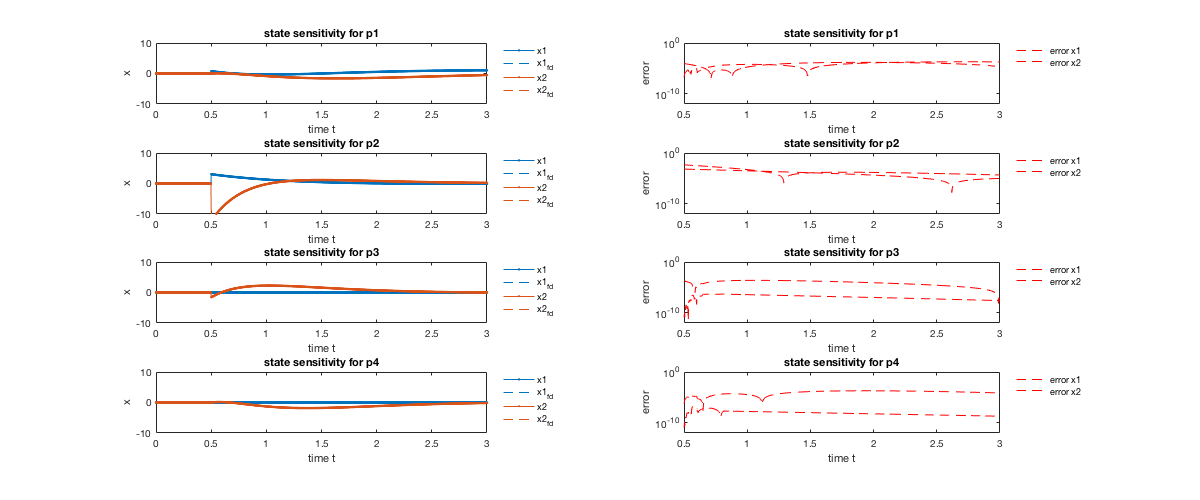
\includegraphics[width=\textwidth]{../../examples/example_dirac_secondorder_vectmult/html/example_dirac_secondorder_vectmult_01.png}

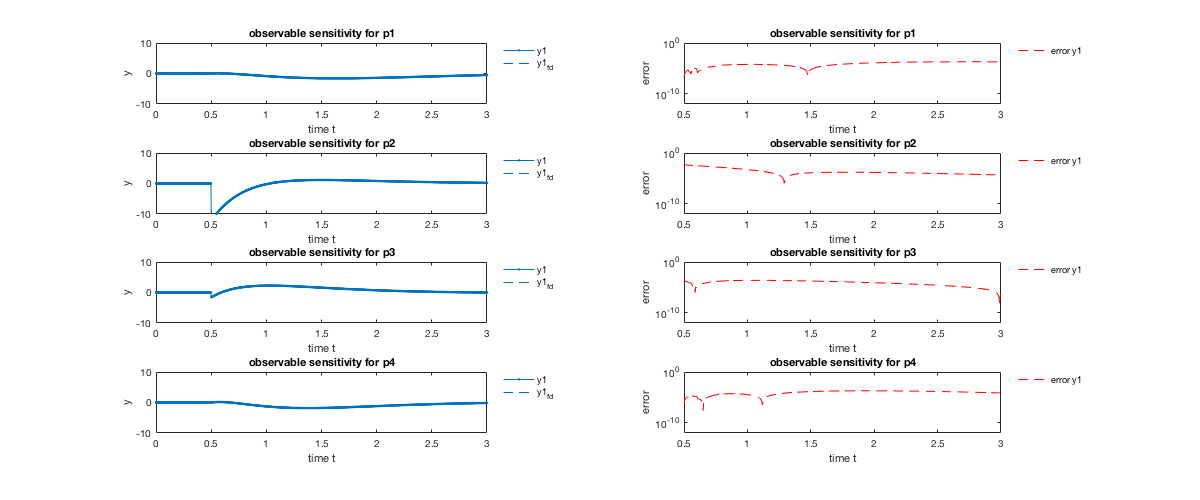
\includegraphics[width=\textwidth]{../../examples/example_dirac_secondorder_vectmult/html/example_dirac_secondorder_vectmult_02.png}
\begin{DoxyCode}
end
\end{DoxyCode}




     \hypertarget{example_adjoint}{}\subsection{Example Adjoint}\label{example_adjoint}
\hypertarget{example_adjoint_def_adjoint}{}\subsubsection{Model Definition}\label{example_adjoint_def_adjoint}
 
% This LaTeX was auto-generated from MATLAB code.
% To make changes, update the MATLAB code and republish this document.











    
    \begin{DoxyCode}
function [model] = model_adjoint_syms()
\end{DoxyCode}
\begin{par}
STATES
\end{par} \vspace{1em}
\begin{DoxyCode}
% create state syms
syms x1

% create state vector
model.sym.x = [x1];
\end{DoxyCode}
\begin{par}
PARAMETERS ( for these sensitivities will be computed )
\end{par} \vspace{1em}
\begin{DoxyCode}
% create parameter syms
syms p1 p2 p3

% create parameter vector
model.sym.p = [p1 p2 p3];


% set the parametrisation of the problem options are 'log', 'log10' and
% 'lin' (default).
model.param = 'log10';
\end{DoxyCode}
\begin{par}
SYSTEM EQUATIONS
\end{par} \vspace{1em}
\begin{DoxyCode}
% create symbolic variable for time
syms t

model.sym.xdot = sym(zeros(size(model.sym.x)));

% piecewise defined function
model.sym.xdot(1) = -p1*x1*heaviside(t-2) + p2;
\end{DoxyCode}
\begin{par}
INITIAL CONDITIONS
\end{par} \vspace{1em}
\begin{DoxyCode}
model.sym.x0 = sym(zeros(size(model.sym.x)));

model.sym.x0(1) = p3;
\end{DoxyCode}
\begin{par}
OBSERVALES
\end{par} \vspace{1em}
\begin{DoxyCode}
model.sym.y = sym(zeros(1,1));

model.sym.y(1) = x1;
\end{DoxyCode}
\begin{DoxyCode}
end
\end{DoxyCode}

         \begin{DoxyCode}ans = 
      sym: [1x1 struct]
    param: 'log10'
\end{DoxyCode} 
    



    \hypertarget{example_adjoint_simu_adjoint}{}\subsubsection{Simulation}\label{example_adjoint_simu_adjoint}
 
% This LaTeX was auto-generated from MATLAB code.
% To make changes, update the MATLAB code and republish this document.











    
    \begin{DoxyCode}
function example_adjoint()
\end{DoxyCode}
\begin{par}
COMPILATION
\end{par} \vspace{1em}
\begin{DoxyCode}
    [exdir,~,~]=fileparts(which('example_adjoint.m'));
    % compile the model
    amiwrap('model_adjoint','model_adjoint_syms',exdir)
\end{DoxyCode}

         \begin{DoxyCode}Generating model struct ...
Parsing model struct ...

Generating C code ...
headers | wrapfunctions | 
Compiling mex file ...
amici | Building with 'Xcode with Clang'.
MEX completed successfully.
Building with 'Xcode with Clang'.
MEX completed successfully.
\end{DoxyCode} 
    \begin{par}
SIMULATION
\end{par} \vspace{1em}
\begin{DoxyCode}
    % time vector
    t = [linspace(0,4,5)];
    p = [1.1,0.3,1];
    k = [];

    D.Y = [     1.0171
        1.3423
        1.6585
        0.9814
        0.3288];

    D.Sigma_Y = 0.1*ones(size(D.Y));


    options.sensi = 1;
    options.sensi_meth = 'adjoint';
    options.maxsteps = 1e4;
    options.rtol = 1e-12;
    options.atol = 1e-12;
    % load mex into memory
    [~] = which('simulate_model_adjoint'); % fix for inaccessability problems
    sol = simulate_model_adjoint(t,log10(p),k,D,options);
\end{DoxyCode}
\begin{par}
Plot
\end{par} \vspace{1em}
\begin{DoxyCode}
    figure
    subplot(3,1,1)
    errorbar(t,D.Y,D.Sigma_Y)
    hold on
    % plot(t,sol.y)

    xlabel('time t')
    ylabel('observable')
    title(['log-likelihood: ' num2str(sol.llh) ])

    y = (p(2)*t + p(3)).*(t<2) + ( (2*p(2)+p(3)-p(2)/p(1))*exp(-p(1)*(t-2))+p(2)/p(1) ).*(t>=2);


    tfine = linspace(0,4,100001);
    xfine = (p(2)*tfine + 1).*(tfine<2) + ( (2*p(2)+p(3)-p(2)/p(1))*exp(-p(1)*(tfine-2))+p(2)/p(1) ).*(tfine>=2);

    mu = zeros(1,length(tfine));
    for it = 1:length(t)
        if(t(it)<=2)
            mu = mu + ((y(it)-D.Y(it))/(D.Sigma_Y(it)^2))*(tfine<=t(it));
        else
            mu = mu + ((y(it)-D.Y(it))/(D.Sigma_Y(it)^2))*exp(p(1)*(tfine-t(it))).*(tfine<=t(it)).*(tfine>2) + ((y(it)-D.Y(it))/(D.Sigma_Y(it)^2))*exp(p(1)*(2-t(it))).*(tfine<t(it)).*(tfine<=2);
        end
    end
    plot(tfine,xfine)
    legend('data','simulation')
    xlim([min(t)-0.5,max(t)+0.5])
    subplot(3,1,2)
    plot(tfine,mu)
    ylabel('adjoint')
    xlabel('time t')
    xlim([min(t)-0.5,max(t)+0.5])

    subplot(3,1,3)

    plot(fliplr(tfine),-cumsum(fliplr(-mu.*xfine.*(tfine>2)))*p(1)*log(10)*(t(end)/numel(tfine)))
    hold on
    plot(fliplr(tfine),-cumsum(fliplr(mu))*p(2)*log(10)*(t(end)/numel(tfine)))
    plot(tfine,-mu(1)*p(3)*log(10)*(tfine<2))
    xlim([min(t)-0.5,max(t)+0.5])
    ylabel('integral')
    xlabel('time t')

    legend('p1','p2','p3')

    grad(1,1) = -trapz(tfine,-mu.*xfine.*(tfine>2))*p(1)*log(10);
    grad(2,1) = -trapz(tfine,mu)*p(2)*log(10);
    grad(3,1) = -mu(1)*p(3)*log(10);

    plot(zeros(3,1),grad,'ko')
\end{DoxyCode}

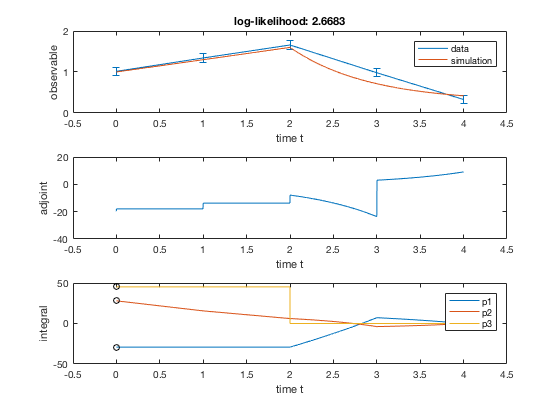
\includegraphics[width=\textwidth]{../../examples/example_adjoint/html/example_adjoint_01.png}
\begin{par}
FD
\end{par} \vspace{1em}
\begin{DoxyCode}
    eps = 1e-5;
    xi = log10(p);
    grad_fd_f = NaN(3,1);
    grad_fd_b = NaN(3,1);
    for ip = 1:3;
        options.sensi = 0;
        xip = xi;
        xip(ip) = xip(ip) + eps;
        solp = simulate_model_adjoint(t,xip,k,D,options);
        grad_fd_f(ip,1) = (solp.llh-sol.llh)/eps;
        xip = xi;
        xip(ip) = xip(ip) - eps;
        solp = simulate_model_adjoint(t,xip,k,D,options);
        grad_fd_b(ip,1) = -(solp.llh-sol.llh)/eps;
    end

    figure
    plot(abs(grad),abs(grad_fd_f),'o')
    hold on
    plot(abs(grad),abs(grad_fd_b),'o')
    plot(abs(grad),mean([abs(grad_fd_b),abs(grad_fd_f)],2),'o')
    plot(abs(grad),abs(sol.sllh),'o')
    plot([1e1,1e2],[1e1,1e2],'k:')
    set(gca,'XScale','log')
    set(gca,'YScale','log')
    axis square
    legend('forward FD','backward FD','central FD','adjoint sensintivity analysis','Location','SouthEast')
    xlabel('analytic absolute value of gradient element')
    ylabel('computed absolute value of gradient element')
    set(gcf,'Position',[100 300 1200 500])

    drawnow
\end{DoxyCode}

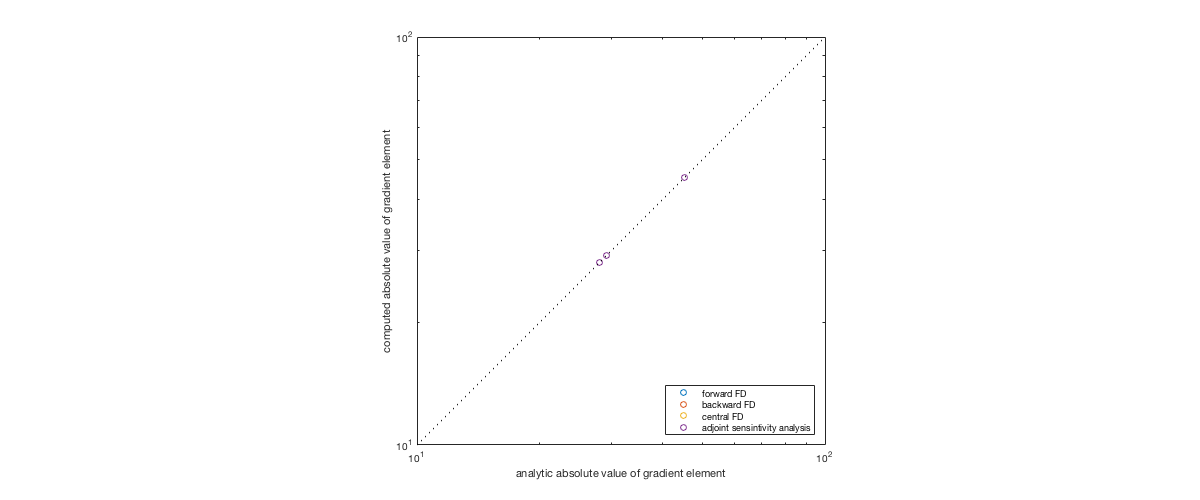
\includegraphics[width=\textwidth]{../../examples/example_adjoint/html/example_adjoint_02.png}
\begin{DoxyCode}
end
\end{DoxyCode}




     